% ============================================================
% PART 1: Preamble, Title Page, Student Details, Sec 1 & 2
% ============================================================
\documentclass[12pt,a4paper]{article}

% --- Packages ---
\usepackage[a4paper, top=1in, bottom=1in, left=1.25in, right=1in]{geometry}
\usepackage{graphicx}
\usepackage{booktabs}
\usepackage{tabularx}
\usepackage{longtable}
\usepackage{array}
\usepackage{multirow}
\usepackage{amsmath}
\usepackage{amssymb}
\usepackage{listings}
\usepackage{xcolor}
\usepackage{hyperref}
\usepackage{fancyhdr}
\usepackage{titlesec}
\usepackage{caption}
\usepackage{subcaption}
\usepackage{setspace}
\usepackage{parskip}
\usepackage{tikz}
\usepackage{pgfplots}
\pgfplotsset{compat=1.18}
\usetikzlibrary{shapes.geometric, arrows.meta, positioning, fit, backgrounds, calc}
\usepackage{enumitem}
\usepackage{float}
\usepackage{microtype}
\usepackage{fontenc}
\usepackage{inputenc}
\usepackage{lmodern}

% --- Hyperref setup ---
\hypersetup{
    colorlinks=true,
    linkcolor=blue!70!black,
    citecolor=green!50!black,
    urlcolor=blue!80!black,
    pdftitle={AES-128 FPGA Image Encryption IP Core},
    pdfauthor={Tanmay Rawal}
}

% --- Header/Footer ---
\pagestyle{fancy}
\fancyhf{}
\fancyhead[L]{\small AES-128 FPGA Image Encryption IP Core}
\fancyhead[R]{\small Tanmay Rawal | 23DEC511}
\fancyfoot[C]{\thepage}
\renewcommand{\headrulewidth}{0.4pt}

% --- Section title formatting ---
\titleformat{\section}{\large\bfseries\color{blue!70!black}}{{\thesection.}}{0.5em}{}[\titlerule]
\titleformat{\subsection}{\normalsize\bfseries\color{blue!50!black}}{{\thesubsection}}{0.5em}{}

% --- Code listing style ---
\lstdefinestyle{verilogstyle}{
    language=Verilog,
    backgroundcolor=\color{gray!8},
    basicstyle=\ttfamily\footnotesize,
    keywordstyle=\color{blue!80!black}\bfseries,
    commentstyle=\color{green!50!black}\itshape,
    stringstyle=\color{red!70!black},
    numberstyle=\tiny\color{gray},
    numbers=left,
    stepnumber=1,
    frame=single,
    breaklines=true,
    captionpos=b,
    tabsize=4,
    showstringspaces=false
}
\lstdefinestyle{cstyle}{
    language=C,
    backgroundcolor=\color{gray!8},
    basicstyle=\ttfamily\footnotesize,
    keywordstyle=\color{blue!80!black}\bfseries,
    commentstyle=\color{green!50!black}\itshape,
    stringstyle=\color{red!70!black},
    numberstyle=\tiny\color{gray},
    numbers=left,
    stepnumber=1,
    frame=single,
    breaklines=true,
    captionpos=b,
    tabsize=4,
    showstringspaces=false
}
\lstdefinestyle{tclstyle}{
    language=tcl,
    backgroundcolor=\color{gray!8},
    basicstyle=\ttfamily\footnotesize,
    keywordstyle=\color{purple!80!black}\bfseries,
    commentstyle=\color{green!50!black}\itshape,
    numberstyle=\tiny\color{gray},
    numbers=left,
    frame=single,
    breaklines=true,
    captionpos=b,
    tabsize=4,
    showstringspaces=false
}

% --- Path for images ---
\graphicspath{{./}}

% ============================================================
\begin{document}

% ============================================================
% TITLE PAGE
% ============================================================
\begin{titlepage}
\centering

\vspace*{0.5cm}

{\LARGE\bfseries Design, FPGA Implementation and Analysis of\\[0.4em]
an AES-128 Image Encryption IP Core\\[0.4em]
on Nexys 4 DDR\par}

\vspace{1.5cm}

{\normalsize Project report submitted in partial fulfillment\\
of the requirements for the degree of\par}

\vspace{0.8cm}

{\large\itshape Bachelor of Technology\\
in\\
Electronics and Communication Engineering\par}

\vspace{1.2cm}

{\normalsize by\par}

\vspace{0.5cm}

{\large\bfseries Tanmay Rawal\\
Roll No-23DEC511\par}

\vspace{0.8cm}

{\normalsize Under Guidance of\par}
\vspace{0.3cm}
{\large\bfseries Dr.\ Kusum Lata\\}
{\normalsize Professor\\
Electronics and Communication Engineering\par}

\vspace{1.2cm}


\includegraphics[width=5cm]{lnmiit_logo.png}

\vspace{1cm}

{\normalsize Department of Electronics and Communication Engineering\\
The LNM Institute of Information Technology, Jaipur\par}

\vspace{1.0cm}

{\large April 27, 2026}

\end{titlepage}

% ============================================================
% STUDENT DETAILS
% ============================================================
\newpage
\thispagestyle{plain}
\vspace*{1cm}

{\large\bfseries\color{blue!70!black} Student Details}\\[0.5em]
\begin{tabular}{ll}
\toprule
\textbf{Field} & \textbf{Detail} \\
\midrule
Name            & Tanmay Rawal \\
Roll Number     & 23DEC511 \\
Department      & Electronics and Communication Engineering \\
Email           & 23dec511@lnmiit.ac.in \\
Programme       & Bachelor of Technology (B.Tech) \\
Institution     & The LNM Institute of Information Technology, Jaipur \\
Project Guide   & Dr.\ Kusum Lata, Professor, ECE \\
Submission Date & April 27, 2026 \\
\bottomrule
\end{tabular}

\vspace{2cm}

% ============================================================
% TABLE OF CONTENTS
% ============================================================
\newpage
\tableofcontents
\newpage
\listoffigures
\newpage

% ============================================================
% SECTION 1: OBJECTIVE
% ============================================================
\section{Objective}

The primary objective of this project is to \textbf{design, implement, and validate a custom AES-128 (Advanced Encryption Standard -- 128-bit key) hardware IP core} for real-time image encryption on the Digilent Nexys 4 DDR FPGA board.

\subsection{Primary Goals}

\begin{enumerate}[leftmargin=*]
    \item \textbf{RTL Design:} Implement a fully FIPS-197 compliant AES-128 encryption engine in Verilog-2001, complete with combinational key expansion, S-box lookup, and all four round operations (SubBytes, ShiftRows, MixColumns, AddRoundKey).
    
    \item \textbf{AXI4-Lite Integration:} Wrap the AES core with an AXI4-Lite slave interface to enable seamless integration into a Xilinx MicroBlaze soft-processor SoC, exposing all cryptographic registers via a memory-mapped register file.
    
    \item \textbf{Hardware-Software Co-Design:} Develop embedded C firmware on the MicroBlaze processor that implements AES-128 in \textbf{Counter (CTR) mode} to encrypt a 64$\times$64 pixel (4,096 byte) grayscale image across 256 blocks in real time.
    
    \item \textbf{JTAG-Based Validation:} Establish a non-intrusive, JTAG-only memory extraction pipeline using Xilinx XSCT scripting to bypass physical UART hardware limitations and directly inspect on-chip BRAM contents.
    
    \item \textbf{Cryptographic Analysis Dashboard:} Build a fully automated real-time HTML visualization dashboard using Python and JavaScript that extracts hardware memory, renders plaintext and ciphertext images side-by-side, and performs NIST-level statistical randomness tests.
    
    \item \textbf{Statistical Verification:} Quantitatively verify the security of the hardware output using Shannon Entropy, Bit Balance, Chi-Square Goodness-of-Fit, pixel distribution histograms, and keystream extraction.
\end{enumerate}

\subsection{Expected Outcomes}

\begin{itemize}[leftmargin=*]
    \item A working AES-128 IP core on silicon achieving 12-cycle latency per 128-bit block.
    \item Measured ciphertext entropy $\geq$ 7.90 bits/byte (theoretical maximum: 8.0).
    \item Near-perfect bit balance ($\approx$50\% ones, 50\% zeros) in the ciphertext.
    \item Chi-Square score close to the ideal value of 255.0 for a uniform distribution over 256 symbols.
    \item A complete, reproducible validation workflow runnable with a single Python command.
\end{itemize}

% ============================================================
% SECTION 2: TOOLS AND RESOURCES USED
% ============================================================
\section{Tools and Resources Used}

\subsection{Development Hardware}

\begin{table}[H]
\centering
\caption{Hardware Platform Specifications}
\begin{tabularx}{\textwidth}{lX}
\toprule
\textbf{Item} & \textbf{Specification} \\
\midrule
Development Board      & Digilent Nexys 4 DDR \\
FPGA Device            & Xilinx Artix-7, xc7a100tcsg324-1, Speed Grade -1 \\
Logic Cells            & 101,440 \\
Look-Up Tables (LUTs)  & 63,400 \\
Flip-Flops             & 126,800 \\
Block RAM              & 4,860 Kb (135 × 36Kb tiles) \\
DSP Slices             & 240 \\
System Clock           & 100 MHz (on-board oscillator) \\
I/O Interface          & USB-UART via FT2232HQ, JTAG via USB \\
On-Board Memory        & 128 MB DDR2 RAM \\
\bottomrule
\end{tabularx}
\end{table}

\subsection{Design Software}

\begin{table}[H]
\centering
\caption{Software Tools Used}
\begin{tabularx}{\textwidth}{lX}
\toprule
\textbf{Tool} & \textbf{Purpose} \\
\midrule
Vivado 2024.2           & FPGA synthesis, implementation, bitstream generation, block design \\
Vitis 2024.2            & Embedded C software development, application build, FPGA programming \\
XSCT (Xilinx Software Command-line Tool) & JTAG-based memory read/write, hardware debugging \\
Python 3.x (Anaconda)   & Dashboard automation, BRAM data extraction, HTML generation \\
Web Browser             & Real-time cryptographic analysis dashboard rendering \\
\bottomrule
\end{tabularx}
\end{table}

\subsection{Languages Used}

\begin{itemize}[leftmargin=*]
    \item \textbf{Verilog-2001} --- RTL design of AES-128 core and AXI4-Lite wrapper
    \item \textbf{C (C99)} --- MicroBlaze embedded firmware (CTR mode encryption, GPIO control)
    \item \textbf{Tcl} --- XSCT automation scripts (BRAM load, memory dump, verification)
    \item \textbf{Python 3} --- Dashboard automation, base64 encoding, HTML generation
    \item \textbf{HTML / CSS / JavaScript} --- Real-time cryptographic analysis dashboard
\end{itemize}

\subsection{IP Cores Used}

\begin{table}[H]
\centering
\caption{Xilinx IP Cores Used in Block Design}
\begin{tabularx}{\textwidth}{llX}
\toprule
\textbf{IP Core} & \textbf{Instance Name} & \textbf{Function} \\
\midrule
MicroBlaze Soft Processor      & microblaze\_0        & 32-bit RISC processor executing CTR encryption firmware \\
AXI Interconnect               & microblaze\_0\_axi\_periph & Routes AXI transactions to peripheral slaves \\
AXI BRAM Controller            & axi\_bram\_ctrl\_0   & Interfaces MicroBlaze to Input BRAM (0xC0000000) \\
AXI BRAM Controller            & axi\_bram\_ctrl\_1   & Interfaces MicroBlaze to Output BRAM (0xC2000000) \\
Block Memory Generator         & blk\_mem\_gen\_0     & 4096-byte Input BRAM (plaintext storage) \\
Block Memory Generator         & blk\_mem\_gen\_1     & 4096-byte Output BRAM (ciphertext storage) \\
AXI GPIO                       & axi\_gpio\_0         & Controls 3 LEDs (status) and reads 2 buttons (BTNC/BTND) \\
AXI UART Lite                  & axi\_uartlite\_0     & UART interface (present in design; bypassed due to pin issue) \\
\textbf{Custom: AES-128 AXI-Lite}  & \textbf{aes128\_axilite\_0} & \textbf{Custom AES-128 encryption IP core (this project)} \\
MicroBlaze Debug Module (MDM)  & mdm\_1               & JTAG-based debug interface \\
Clocking Wizard                & clk\_wiz             & Generates stable system clock from on-board 100 MHz oscillator \\
\bottomrule
\end{tabularx}
\end{table}

% ============================================================
% PART 2: Section 3 - System Design / Architecture
% ============================================================

% ---- SECTION 3 ----
\section{System Design / Architecture}

\subsection{Top-Level System Architecture}

The system follows a \textbf{hardware-software co-design} methodology built around the Xilinx MicroBlaze soft-core processor connected to a custom AES-128 hardware accelerator over an AXI4-Lite bus. Figure~\ref{fig:block_design} shows the Vivado block design.

\begin{figure}[H]
    \centering
    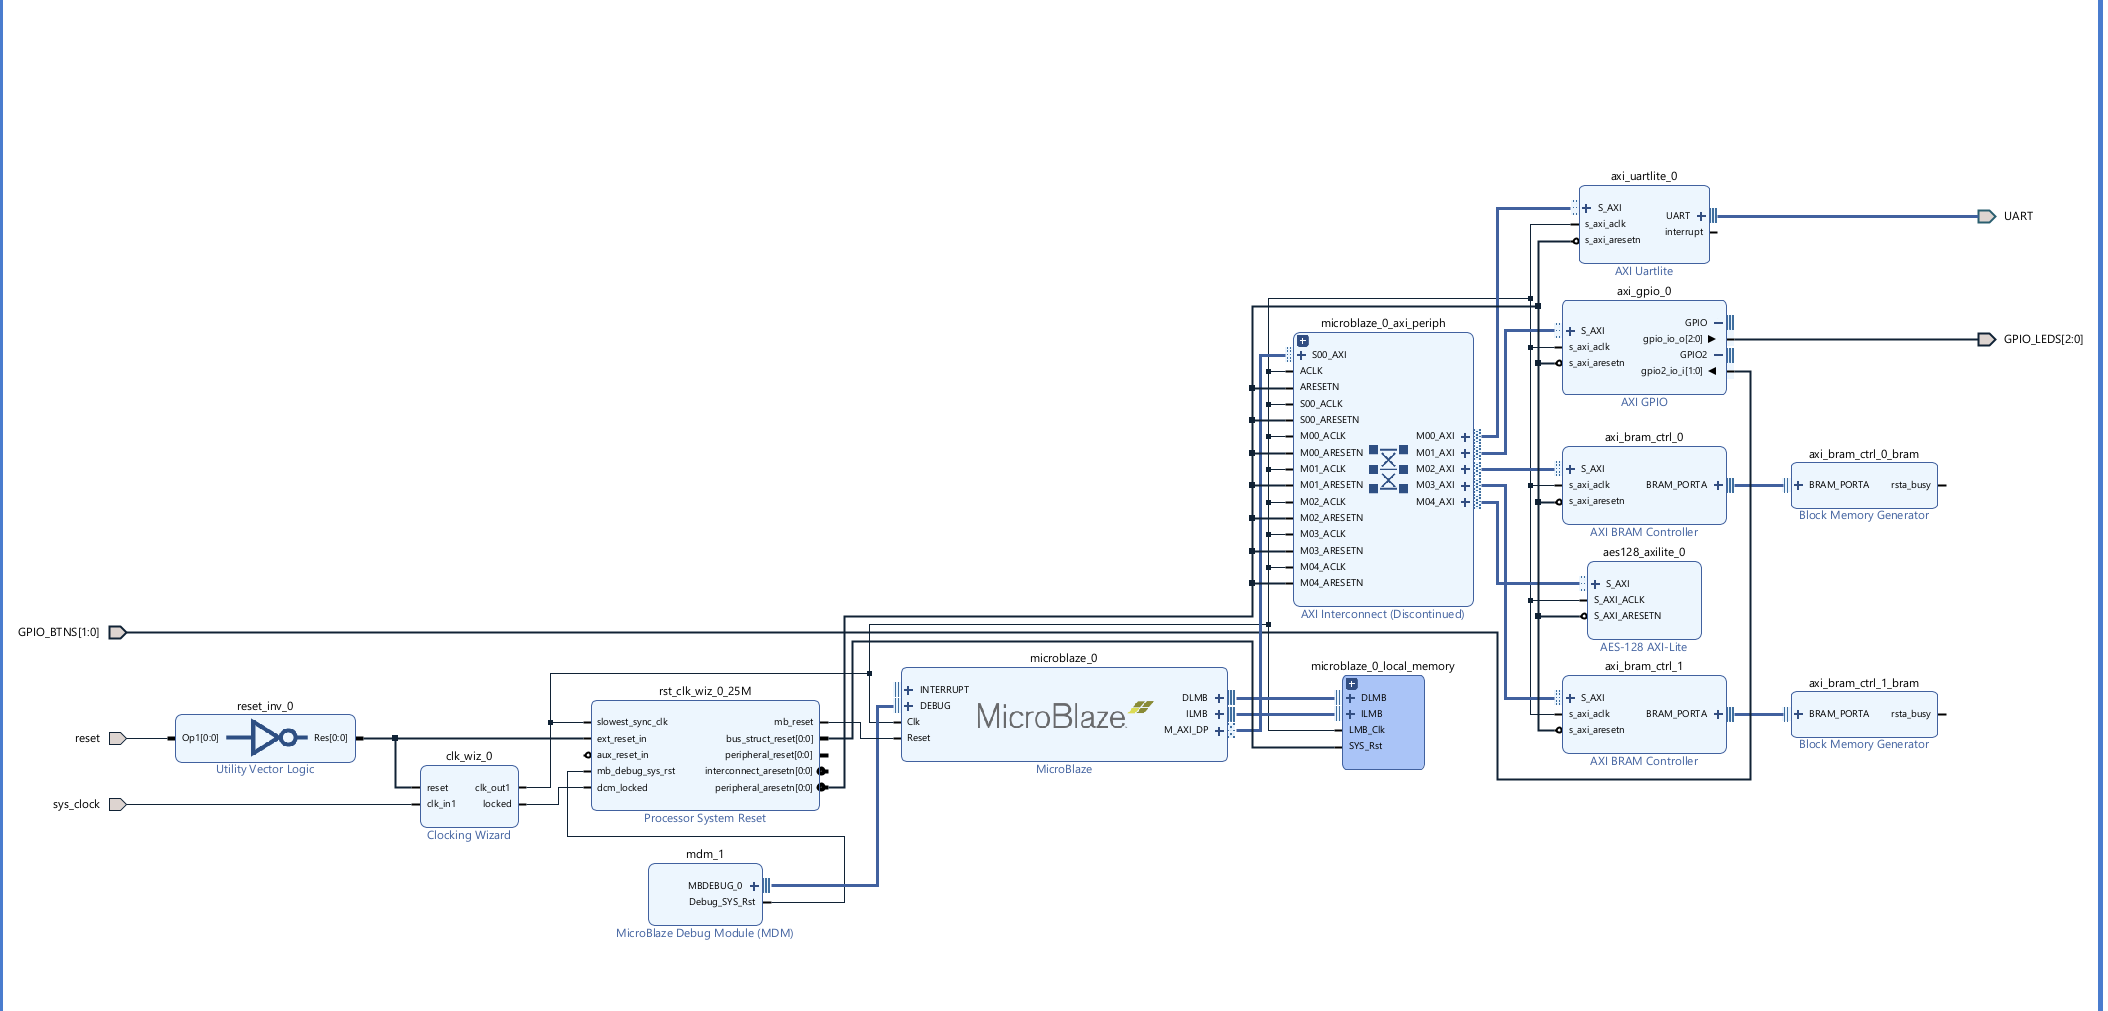
\includegraphics[width=\textwidth]{block_design.png}
    \caption{Vivado Block Design: Full SoC Architecture showing MicroBlaze, AXI Interconnect, Custom AES-128 IP, Dual BRAM Controllers, GPIO, and UART.}
    \label{fig:block_design}
\end{figure}

The architecture diagram (Figure~\ref{fig:arch_tikz}) shows the data flow from a conceptual standpoint.

\begin{figure}[H]
\centering
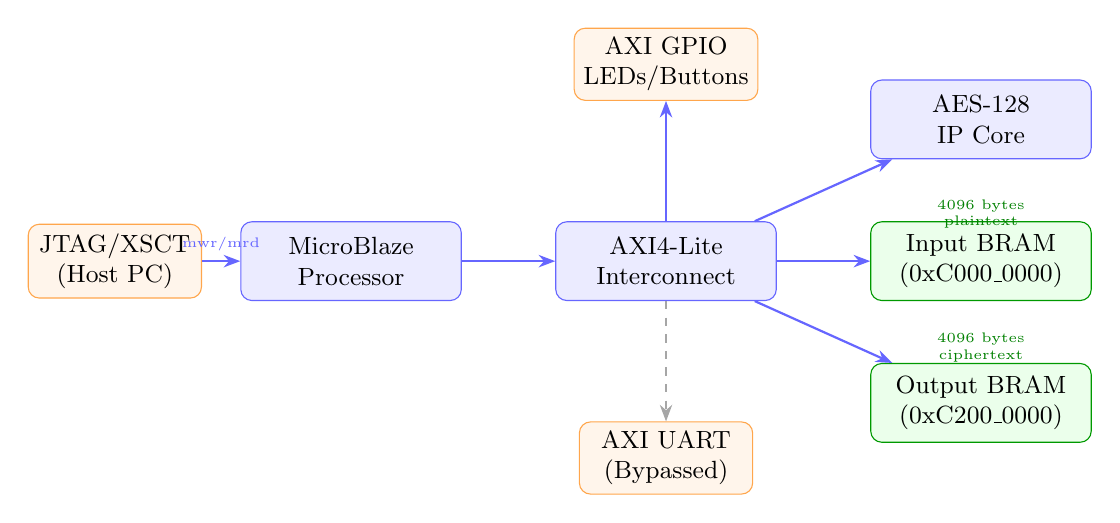
\begin{tikzpicture}[
    block/.style={rectangle, draw=blue!60, fill=blue!8, rounded corners, minimum width=2.8cm, minimum height=1cm, align=center, font=\small},
    memblock/.style={rectangle, draw=green!60!black, fill=green!8, rounded corners, minimum width=2.8cm, minimum height=1cm, align=center, font=\small},
    ioblock/.style={rectangle, draw=orange!70, fill=orange!8, rounded corners, minimum width=2.2cm, minimum height=0.9cm, align=center, font=\small},
    arrow/.style={-{Stealth[length=6pt]}, thick, blue!60},
    dasharrow/.style={-{Stealth[length=6pt]}, dashed, gray!70}
]

\node[block] (mb) at (0,0) {MicroBlaze\\Processor};
\node[block] (axi) at (4,0) {AXI4-Lite\\Interconnect};
\node[block] (aes) at (8,1.8) {AES-128\\IP Core};
\node[memblock] (bram0) at (8,0) {Input BRAM\\(0xC000\_0000)};
\node[memblock] (bram1) at (8,-1.8) {Output BRAM\\(0xC200\_0000)};
\node[ioblock] (gpio) at (4,2.5) {AXI GPIO\\LEDs/Buttons};
\node[ioblock] (uart) at (4,-2.5) {AXI UART\\(Bypassed)};
\node[ioblock] (jtag) at (-3,0) {JTAG/XSCT\\(Host PC)};

\draw[arrow] (mb) -- (axi);
\draw[arrow] (axi) -- (aes);
\draw[arrow] (axi) -- (bram0);
\draw[arrow] (axi) -- (bram1);
\draw[arrow] (axi) -- (gpio);
\draw[dasharrow] (axi) -- (uart);
\draw[arrow] (jtag) -- node[above, font=\tiny]{mwr/mrd} (mb);

\node[font=\tiny, text=green!50!black, align=center] at (8,0.6) {4096 bytes\\plaintext};
\node[font=\tiny, text=green!50!black, align=center] at (8,-1.1) {4096 bytes\\ciphertext};

\end{tikzpicture}
\caption{Conceptual System Architecture Block Diagram}
\label{fig:arch_tikz}
\end{figure}

\subsection{Memory Map}

\begin{table}[H]
\centering
\caption{System Memory Map}
\begin{tabular}{llll}
\toprule
\textbf{Peripheral} & \textbf{Base Address} & \textbf{Size} & \textbf{Purpose} \\
\midrule
Input BRAM (axi\_bram\_ctrl\_0)  & \texttt{0xC000\_0000} & 4 KB & Plaintext image storage \\
Output BRAM (axi\_bram\_ctrl\_1) & \texttt{0xC200\_0000} & 4 KB & Ciphertext storage \\
AES-128 IP (aes128\_axilite\_0)  & \texttt{0x44A0\_0000} & 64 B & AES register interface \\
AXI GPIO (axi\_gpio\_0)          & \texttt{0x4012\_0000} & 64 KB & LED/Button control \\
AXI UART Lite                    & \texttt{0x4060\_0000} & 64 KB & UART (bypassed) \\
\bottomrule
\end{tabular}
\end{table}

\subsection{AES-128 Core Design (\texttt{aes128\_core.v})}

The AES-128 engine is the heart of the IP core. It implements the complete FIPS-197 AES-128 ECB encryption algorithm in synthesizable Verilog-2001.

\subsubsection{Module Port Interface}

\begin{table}[H]
\centering
\caption{AES-128 Core Port Descriptions}
\begin{tabular}{llll}
\toprule
\textbf{Port} & \textbf{Direction} & \textbf{Width} & \textbf{Description} \\
\midrule
\texttt{clk}      & Input  & 1 bit  & System clock (100 MHz) \\
\texttt{rst\_n}   & Input  & 1 bit  & Active-low synchronous reset \\
\texttt{start}    & Input  & 1 bit  & Pulse HIGH for 1 cycle to begin encryption \\
\texttt{key}      & Input  & 128 bit & AES-128 encryption key \\
\texttt{data\_in} & Input  & 128 bit & Plaintext block input \\
\texttt{data\_out}& Output & 128 bit & Ciphertext block output \\
\texttt{done}     & Output & 1 bit  & Pulses HIGH for 1 cycle when output is valid \\
\bottomrule
\end{tabular}
\end{table}

\subsubsection{AES Round Operations}

The core implements all four standard AES round transformations operating on a 4$\times$4 byte state matrix:

\begin{enumerate}[leftmargin=*]
    \item \textbf{SubBytes} --- Each byte of the 128-bit state is substituted using the AES S-box, implemented as a 256-entry combinational \texttt{case} statement in Verilog. The S-box is derived from the multiplicative inverse in GF($2^8$) followed by an affine transformation.
    \item \textbf{ShiftRows} --- Row $r$ of the state matrix is cyclically shifted left by $r$ bytes (row 0: no shift, row 1: 1 byte, row 2: 2 bytes, row 3: 3 bytes), implemented as a combinational byte reorder.
    \item \textbf{MixColumns} --- Each 4-byte column is multiplied by a fixed polynomial matrix in GF($2^8$). The \texttt{xtime} function (left-shift with reduction polynomial $x^8+x^4+x^3+x+1$) is used:
    \begin{equation}
    \begin{bmatrix} r_0 \\ r_1 \\ r_2 \\ r_3 \end{bmatrix}
    =
    \begin{bmatrix} 2 & 3 & 1 & 1 \\ 1 & 2 & 3 & 1 \\ 1 & 1 & 2 & 3 \\ 3 & 1 & 1 & 2 \end{bmatrix}
    \begin{bmatrix} s_0 \\ s_1 \\ s_2 \\ s_3 \end{bmatrix}
    \pmod{x^8+x^4+x^3+x+1}
    \end{equation}
    \item \textbf{AddRoundKey} --- 128-bit XOR of the state with the current round key.
\end{enumerate}

\subsubsection{Key Expansion}

The key schedule generates 11 round keys (W[0]--W[43]) from the 128-bit input key using the \texttt{key\_expand} task. This is implemented \textbf{combinationally} and executes in the first clock cycle when \texttt{start} is asserted, using \texttt{RotWord}, \texttt{SubWord}, and the Rcon constants.

\subsubsection{Finite State Machine}

The AES core uses a simple 3-state FSM (Figure~\ref{fig:fsm_tikz}):

\begin{figure}[H]
\centering
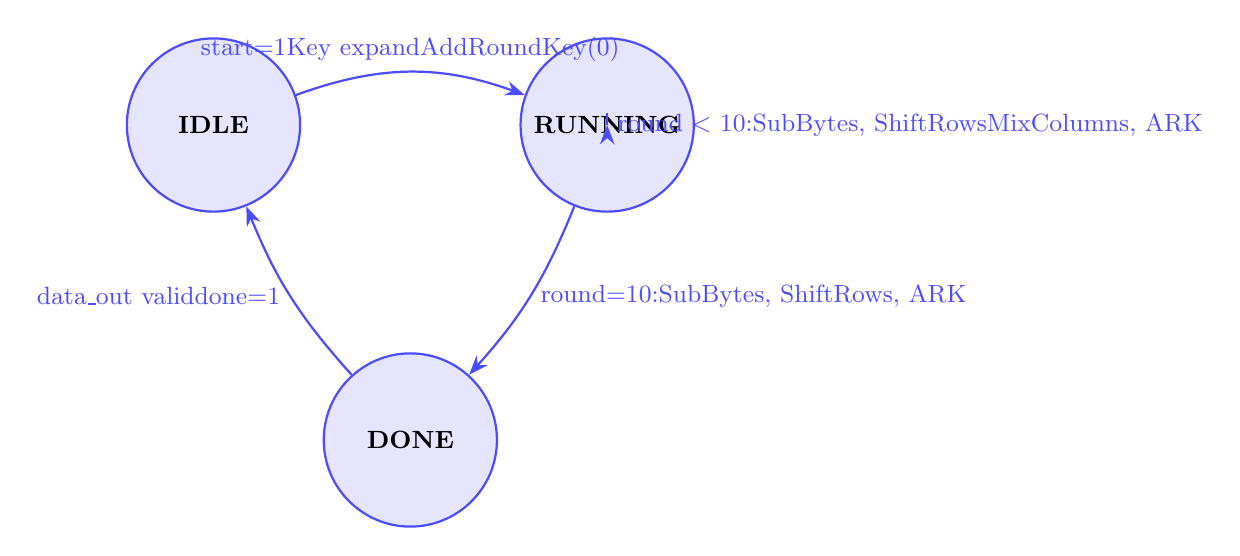
\begin{tikzpicture}[
    state/.style={circle, draw=blue!70, fill=blue!10, thick, minimum size=2.2cm, align=center, font=\small\bfseries},
    arrow/.style={-{Stealth[length=7pt]}, thick, blue!70}
]
\node[state] (idle) at (0,0) {IDLE};
\node[state] (run) at (5,0) {RUNNING};
\node[state] (done) at (2.5,-4) {DONE};

\draw[arrow] (idle) to[bend left=20] node[above, font=\small]{start=1\\Key expand\\AddRoundKey(0)} (run);
\draw[arrow] (run) to[bend left=20] node[right, font=\small]{round $<$ 10:\\SubBytes, ShiftRows\\MixColumns, ARK} (run);
\draw[arrow] (run) to[bend left=10] node[right, font=\small]{round=10:\\SubBytes, ShiftRows, ARK} (done);
\draw[arrow] (done) to[bend left=10] node[left, font=\small]{data\_out valid\\done=1} (idle);
\end{tikzpicture}
\caption{AES Core Finite State Machine (IDLE $\to$ RUNNING $\to$ DONE)}
\label{fig:fsm_tikz}
\end{figure}

\textbf{Latency:} 12 clock cycles total --- 1 cycle for key expansion + initial AddRoundKey, 9 cycles for rounds 1--9 (with MixColumns), 1 cycle for round 10 (no MixColumns), 1 cycle to assert \texttt{done} and latch output.

\subsection{AXI4-Lite Wrapper (\texttt{aes128\_axilite\_wrapper.v})}

The AXI4-Lite wrapper exposes the AES core to the MicroBlaze processor via 14 memory-mapped 32-bit registers.

\subsubsection{AXI4-Lite Register Map}

\begin{table}[H]
\centering
\caption{AXI4-Lite Register Map (Base Address: 0x44A00000)}
\begin{tabular}{lllp{5cm}}
\toprule
\textbf{Offset} & \textbf{Register} & \textbf{R/W} & \textbf{Description} \\
\midrule
\texttt{0x00} & CTRL    & W & bit[0]=START, bit[1]=SOFT\_RST \\
\texttt{0x04} & STATUS  & R & bit[0]=DONE (latched until next START) \\
\texttt{0x08} & KEY\_W0 & W & key[127:96] \\
\texttt{0x0C} & KEY\_W1 & W & key[95:64] \\
\texttt{0x10} & KEY\_W2 & W & key[63:32] \\
\texttt{0x14} & KEY\_W3 & W & key[31:0] \\
\texttt{0x18} & DIN\_W0 & W & data\_in[127:96] \\
\texttt{0x1C} & DIN\_W1 & W & data\_in[95:64] \\
\texttt{0x20} & DIN\_W2 & W & data\_in[63:32] \\
\texttt{0x24} & DIN\_W3 & W & data\_in[31:0] \\
\texttt{0x28} & DOUT\_W0 & R & data\_out[127:96] \\
\texttt{0x2C} & DOUT\_W1 & R & data\_out[95:64] \\
\texttt{0x30} & DOUT\_W2 & R & data\_out[63:32] \\
\texttt{0x34} & DOUT\_W3 & R & data\_out[31:0] \\
\bottomrule
\end{tabular}
\end{table}

\subsection{CTR Mode Block Diagram}

Figure~\ref{fig:ctr_tikz} shows how CTR mode is implemented. The AES core encrypts a counter value (not the plaintext), and the resulting keystream is XOR'd with the plaintext to produce ciphertext --- making it a stream cipher with the security of AES.

\begin{figure}[H]
\centering
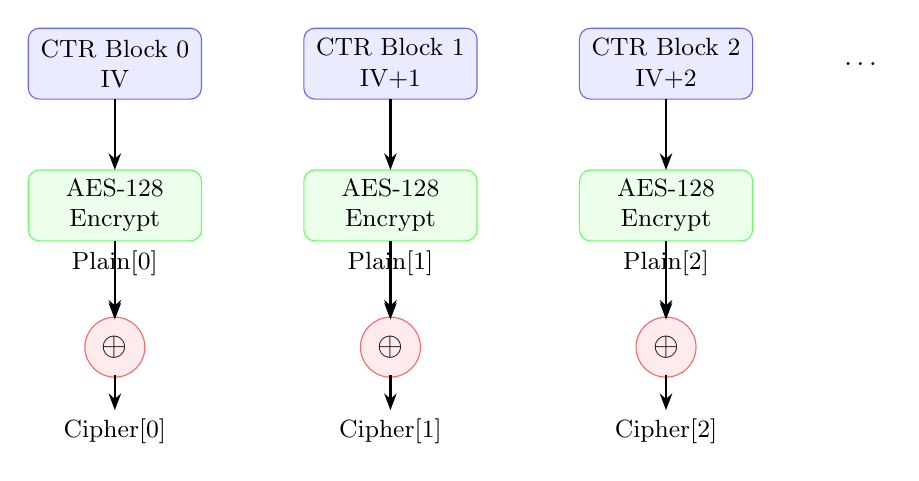
\begin{tikzpicture}[
    block/.style={rectangle, draw=blue!60, fill=blue!8, rounded corners, minimum width=2.2cm, minimum height=0.9cm, align=center, font=\small},
    xornode/.style={circle, draw=red!60, fill=red!8, minimum size=0.7cm, font=\large},
    arrow/.style={-{Stealth[length=6pt]}, thick}
]
\node[block] (ctr0) at (0,0) {CTR Block 0\\IV};
\node[block] (ctr1) at (3.5,0) {CTR Block 1\\IV+1};
\node[block] (ctr2) at (7,0) {CTR Block 2\\IV+2};
\node (dots) at (9.5,0) {\ldots};

\node[block, fill=green!8, draw=green!60] (aes0) at (0,-1.8) {AES-128\\Encrypt};
\node[block, fill=green!8, draw=green!60] (aes1) at (3.5,-1.8) {AES-128\\Encrypt};
\node[block, fill=green!8, draw=green!60] (aes2) at (7,-1.8) {AES-128\\Encrypt};

\node[xornode] (xor0) at (0,-3.6) {$\oplus$};
\node[xornode] (xor1) at (3.5,-3.6) {$\oplus$};
\node[xornode] (xor2) at (7,-3.6) {$\oplus$};

\node[above=0.4cm of xor0, font=\small] (p0) {Plain[0]};
\node[above=0.4cm of xor1, font=\small] (p1) {Plain[1]};
\node[above=0.4cm of xor2, font=\small] (p2) {Plain[2]};

\node[below=0.4cm of xor0, font=\small] (c0) {Cipher[0]};
\node[below=0.4cm of xor1, font=\small] (c1) {Cipher[1]};
\node[below=0.4cm of xor2, font=\small] (c2) {Cipher[2]};

\foreach \x in {0,1,2} {
    \pgfmathparse{int(\x*3.5)}
    \draw[arrow] (\x*3.5, -0.45) -- (\x*3.5,-1.35);
    \draw[arrow] (\x*3.5,-2.25) -- (\x*3.5,-3.25);
    \draw[arrow] (\x*3.5,-3.95) -- (\x*3.5,-4.4);
}
\draw[arrow] (p0) -- (xor0);
\draw[arrow] (p1) -- (xor1);
\draw[arrow] (p2) -- (xor2);

\end{tikzpicture}
\caption{AES-128 CTR Mode Operation: Counter blocks are encrypted to generate a keystream, which is XOR'd with plaintext blocks to produce ciphertext.}
\label{fig:ctr_tikz}
\end{figure}

% ============================================================
% PART 3: Section 4 (Implementation) + Section 5 (Simulation & Testing)
% ============================================================

% ---- SECTION 4 ----
\section{Implementation}

\subsection{Vivado Block Design and IP Packaging}

The hardware implementation was carried out in Vivado 2024.2. The AES-128 core was first packaged as a custom IP using the \textit{Package IP} wizard, creating a \texttt{component.xml} descriptor that registers the AXI4-Lite interface, clock, and reset ports for Vivado's IP Integrator.

The block design (Figure~\ref{fig:block_design}) was constructed by:
\begin{enumerate}[leftmargin=*]
    \item Instantiating a MicroBlaze soft processor with 128 KB local memory.
    \item Running \textit{Run Block Automation} to auto-add the Processor System Reset, MDM debug module, and Clocking Wizard (100 MHz).
    \item Adding the AXI BRAM Controller IP twice for independent Input (0xC0000000) and Output (0xC2000000) BRAMs.
    \item Connecting a 4 KB Block Memory Generator to each BRAM controller.
    \item Adding the custom AES-128 AXI-Lite IP from the user IP repository.
    \item Adding AXI GPIO (3 LED outputs + 2 button inputs) and AXI UART Lite.
    \item Running \textit{Run Connection Automation} to complete all AXI interconnect wiring.
\end{enumerate}

\subsection{Pin Assignments (XDC Constraints)}

The physical I/O pin assignments were defined in the Xilinx Design Constraints (XDC) file \texttt{nexys4ddr\_image\_crypto.xdc}:

\begin{lstlisting}[style=tclstyle, caption={Key XDC Pin Assignments for Nexys 4 DDR}]
# UART
set_property PACKAGE_PIN C4  [get_ports UART_txd]
set_property PACKAGE_PIN D4  [get_ports UART_rxd]
set_property IOSTANDARD LVCMOS33 [get_ports UART_txd]
set_property IOSTANDARD LVCMOS33 [get_ports UART_rxd]

# GPIO LEDs
set_property PACKAGE_PIN H17 [get_ports {GPIO_LEDS[0]}]  ;# LED0 (idle indicator)
set_property PACKAGE_PIN N15 [get_ports {GPIO_LEDS[1]}]  ;# LED16_R (encrypting)
set_property PACKAGE_PIN R11 [get_ports {GPIO_LEDS[2]}]  ;# LED16_G (done)

# GPIO Buttons
set_property PACKAGE_PIN N17 [get_ports {GPIO_BTNS[0]}]  ;# BTNC (trigger)
set_property PACKAGE_PIN P18 [get_ports {GPIO_BTNS[1]}]  ;# BTND
\end{lstlisting}

\subsection{Firmware Implementation (\texttt{main.c})}

The embedded C firmware implements the complete AES-128 CTR mode encryption loop. The firmware was built in Vitis 2024.2 targeting the MicroBlaze BSP (standalone domain).

\subsubsection{Cryptographic Parameters}

\begin{itemize}[leftmargin=*]
    \item \textbf{Key (128-bit):} \texttt{00 01 02 03 04 05 06 07 08 09 0A 0B 0C 0D 0E 0F}
    \item \textbf{IV / Initial Counter (128-bit):} \texttt{F0 E0 D0 C0 B0 A0 90 80 70 60 50 40 30 20 01 00}
    \item \textbf{Image Size:} 64$\times$64 pixels = 4096 bytes = 256 AES blocks
\end{itemize}

\subsubsection{LED State Machine}

The firmware uses three GPIO-controlled LEDs to visually indicate the encryption state:

\begin{figure}[H]
\centering
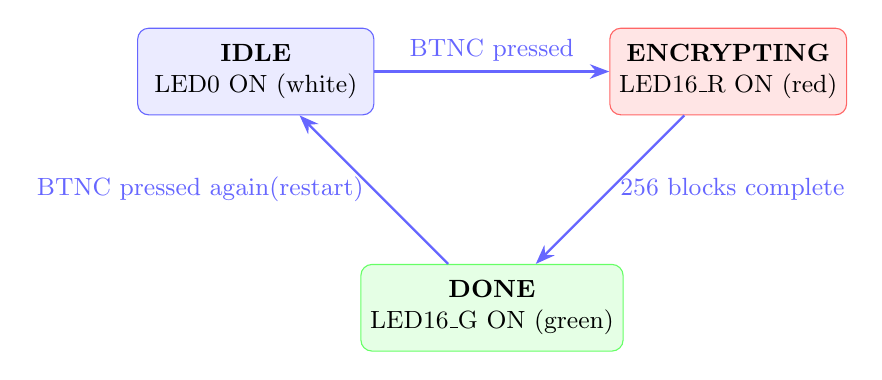
\begin{tikzpicture}[
    state/.style={rectangle, draw=blue!60, fill=blue!8, rounded corners, minimum width=3cm, minimum height=1.1cm, align=center, font=\small},
    arrow/.style={-{Stealth[length=7pt]}, thick, blue!60}
]
\node[state] (idle) at (0,0) {\textbf{IDLE}\\LED0 ON (white)};
\node[state, fill=red!10, draw=red!60] (enc) at (6,0) {\textbf{ENCRYPTING}\\LED16\_R ON (red)};
\node[state, fill=green!10, draw=green!60] (done) at (3,-3) {\textbf{DONE}\\LED16\_G ON (green)};

\draw[arrow] (idle) -- node[above, font=\small]{BTNC pressed} (enc);
\draw[arrow] (enc) -- node[right, font=\small]{256 blocks complete} (done);
\draw[arrow] (done) -- node[left, font=\small]{BTNC pressed again\\(restart)} (idle);
\end{tikzpicture}
\caption{Firmware LED State Machine: LED0=Idle, Red=Encrypting, Green=Done}
\label{fig:led_fsm}
\end{figure}

\subsubsection{Core Encryption Loop}

\begin{lstlisting}[style=cstyle, caption={CTR Mode Encryption Loop (from main.c)}]
/* Write key to AES IP */
AES_WriteKey(key);

for (uint32_t blk = 0; blk < 256; blk++) {
    uint32_t byte_off = blk * 16;

    /* 1. Read plaintext block from Input BRAM */
    for (int i = 0; i < 4; i++) {
        uint32_t w = Xil_In32(XPAR_AXI_BRAM_CTRL_0_BASEADDR + byte_off + i*4);
        plain[i*4+0] = (w >> 24) & 0xFF;
        plain[i*4+1] = (w >> 16) & 0xFF;
        plain[i*4+2] = (w >>  8) & 0xFF;
        plain[i*4+3] =  w        & 0xFF;
    }

    /* 2. Encrypt counter to get keystream block */
    AES_WriteDataIn(counter);
    AES_Start();
    AES_WaitDone();   /* Poll STATUS[0] until DONE=1 (12 cycles) */
    AES_ReadDataOut(ks);

    /* 3. XOR keystream with plaintext -> ciphertext */
    for (int i = 0; i < 16; i++)
        cipher[i] = plain[i] ^ ks[i];

    /* 4. Write ciphertext to Output BRAM */
    for (int i = 0; i < 4; i++) {
        uint32_t w = ((uint32_t)cipher[i*4+0] << 24) |
                     ((uint32_t)cipher[i*4+1] << 16) |
                     ((uint32_t)cipher[i*4+2] <<  8) |
                     ((uint32_t)cipher[i*4+3]);
        Xil_Out32(XPAR_AXI_BRAM_CTRL_1_BASEADDR + byte_off + i*4, w);
    }

    /* 5. Increment counter (big-endian) */
    for (int j = 15; j >= 0; j--)
        if (++counter[j] != 0x00) break;
}
\end{lstlisting}

\subsubsection{AES IP Software Driver (\texttt{aes\_ip\_driver.h})}

The driver provides inline C functions that abstract all AXI register read/write operations:

\begin{lstlisting}[style=cstyle, caption={Key AES IP Driver Functions (aes\_ip\_driver.h)}]
/* Poll STATUS register until DONE bit is set */
static inline void AES_WaitDone(void) {
    while (!(AES_READ(AES_REG_STATUS) & AES_STATUS_DONE)) { /* poll */ }
}

/* Pulse the START bit to begin encryption */
static inline void AES_Start(void) {
    AES_WRITE(AES_REG_CTRL, AES_CTRL_START);
}
\end{lstlisting}

\subsection{Vivado Project Screenshots}

\begin{figure}[H]
    \centering
    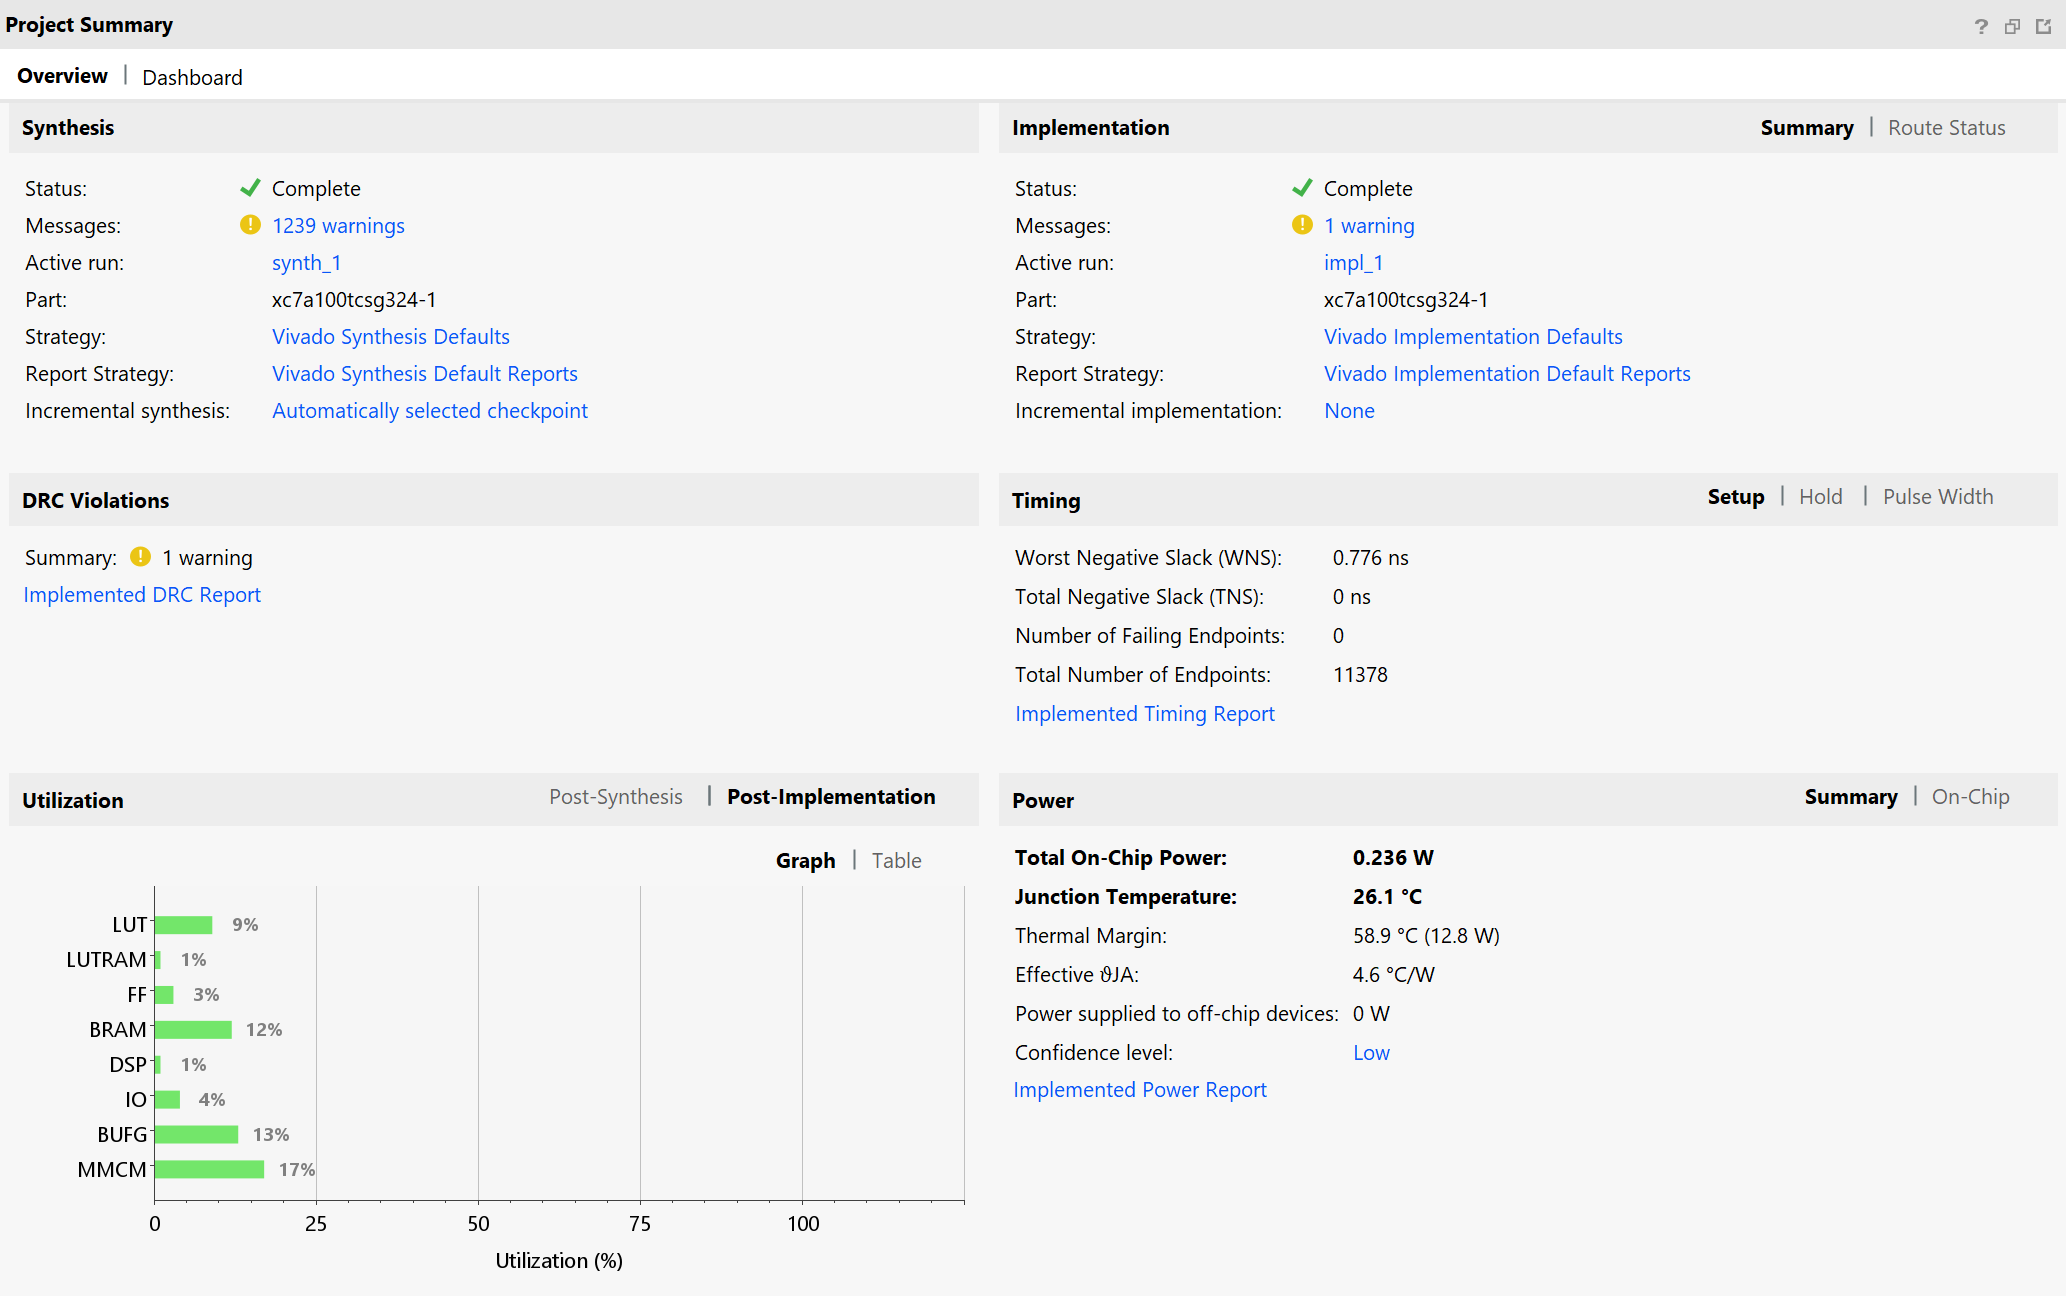
\includegraphics[width=0.9\textwidth]{project_summary.png}
    \caption{Vivado Project Summary showing design status, device, and implementation results.}
    \label{fig:proj_summary}
\end{figure}

\begin{figure}[H]
    \centering
    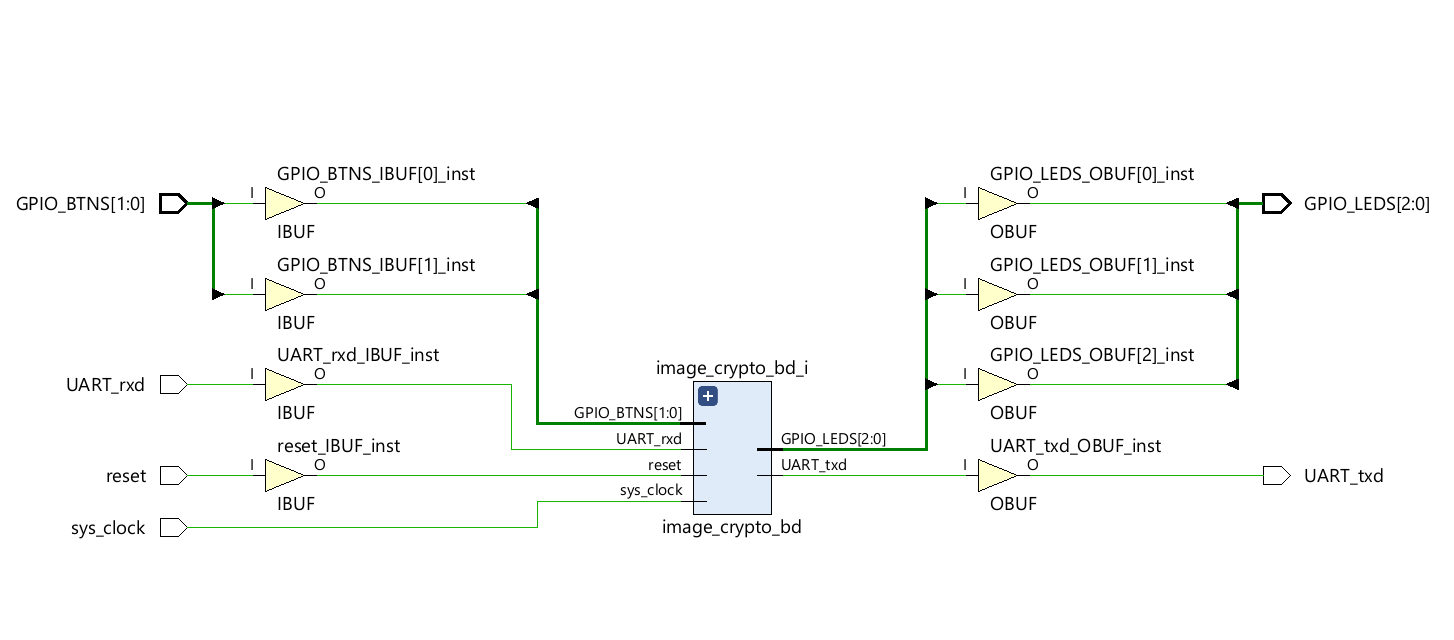
\includegraphics[width=\textwidth]{schematic.png}
    \caption{Post-Implementation Schematic View showing synthesized logic.}
    \label{fig:schematic}
\end{figure}

\begin{figure}[H]
    \centering
    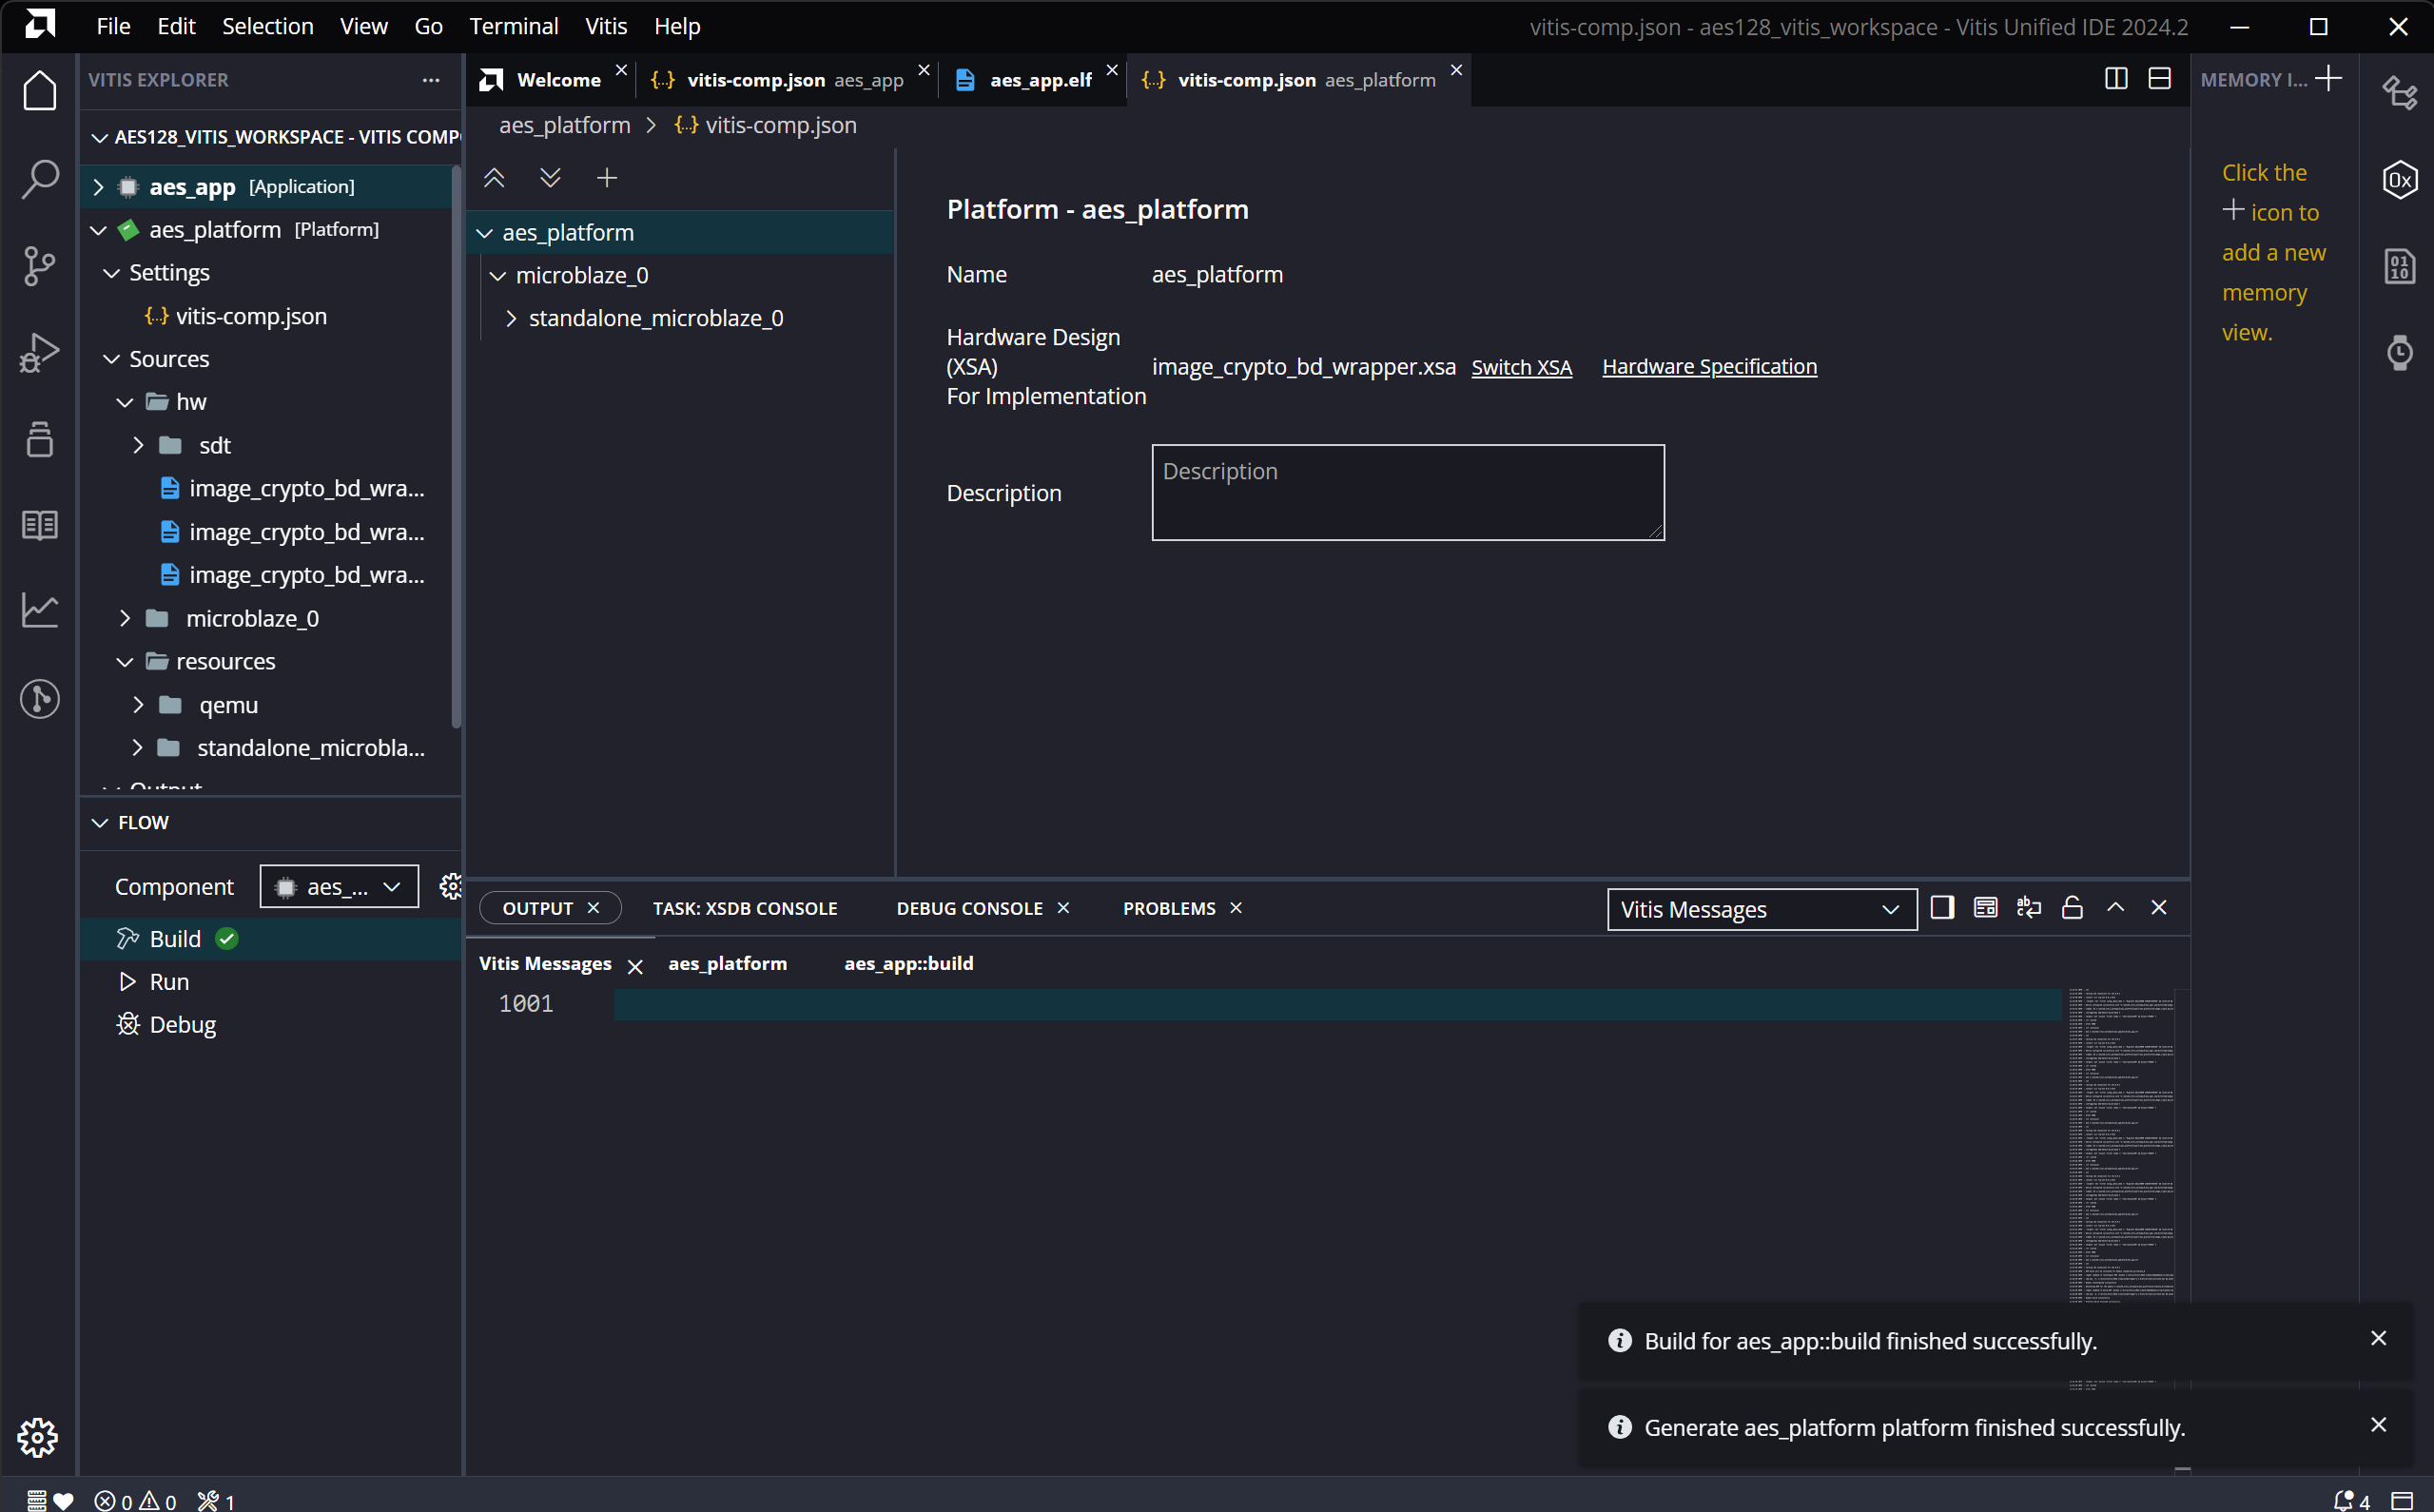
\includegraphics[width=0.85\textwidth]{vitis_project.png}
    \caption{Vitis 2024.2 IDE showing the \texttt{aes\_app} project structure with \texttt{main.c} and \texttt{aes\_ip\_driver.h}.}
    \label{fig:vitis}
\end{figure}

% ---- SECTION 5 ----
\section{Simulation and Testing}

\subsection{On-Board Testing Procedure}

Due to the UART hardware constraint (detailed in Section~\ref{sec:challenges}), all testing was performed via JTAG-based direct memory access. The complete on-board testing workflow is illustrated in Figure~\ref{fig:workflow}.

\begin{figure}[H]
\centering
\begin{tikzpicture}[
    step/.style={rectangle, draw=blue!60, fill=blue!8, rounded corners, minimum width=4cm, minimum height=0.9cm, align=center, font=\small},
    hw/.style={rectangle, draw=green!60, fill=green!8, rounded corners, minimum width=4cm, minimum height=0.9cm, align=center, font=\small},
    arrow/.style={-{Stealth[length=7pt]}, thick}
]
\node[step] (s1) at (0,0)   {1. Run AES App in Vitis\\(Programs FPGA + ELF)};
\node[step] (s2) at (0,-1.6){2. Run \texttt{auto\_dashboard.py}\\(Launches Python script)};
\node[step] (s3) at (0,-3.2){3. XSCT: Load 4096-byte\\gradient image via JTAG \texttt{mwr}};
\node[hw]   (s4) at (0,-4.8){4. User presses BTNC\\on Nexys 4 DDR board};
\node[hw]   (s5) at (0,-6.4){5. MicroBlaze: Encrypt 256\\blocks (Green LED = Done)};
\node[step] (s6) at (0,-8.0){6. User presses ENTER\\in Python terminal};
\node[step] (s7) at (0,-9.6){7. XSCT: Dump both BRAMs\\to \texttt{input\_image.raw} and \\ \texttt{output\_image.raw}};
\node[step] (s8) at (0,-11.2){8. Python: Generates HTML\\dashboard with analysis};

\foreach \a/\b in {s1/s2, s2/s3, s3/s4, s4/s5, s5/s6, s6/s7, s7/s8}
    \draw[arrow] (\a) -- (\b);
\end{tikzpicture}
\caption{Complete End-to-End Testing and Validation Workflow}
\label{fig:workflow}
\end{figure}

\subsection{Test Image Injection via JTAG}

A 64$\times$64 grayscale gradient image (4,096 bytes) was used as the test input. Since UART was bypassed, the image was injected directly into the Input BRAM at \texttt{0xC0000000} using an auto-generated Tcl script containing 1,024 individual \texttt{mwr} commands:

\begin{lstlisting}[style=tclstyle, caption={JTAG Memory Write Script (load\_explicit.tcl) Excerpt}]
connect
targets -set -filter {name =~ "MicroBlaze #0"}
mwr 0xC0000000 0xA0A0A0A0
mwr 0xC0000004 0xA0A0A0A0
...
mwr 0xC0000FFC 0xA0A0A0A0
disconnect
\end{lstlisting}

\subsection{Memory Extraction via JTAG}

After encryption (confirmed by solid Green LED), both BRAMs were read back using the \texttt{dump\_both.tcl} script which saves 4,096 bytes from each BRAM into binary raw files for analysis.

\subsection{Observed vs Expected Behaviour}

\begin{table}[H]
\centering
\caption{Simulation and Testing: Observed vs Expected Behaviour}
\begin{tabularx}{\textwidth}{lXX}
\toprule
\textbf{Test} & \textbf{Expected Behaviour} & \textbf{Observed Behaviour} \\
\midrule
LED Idle State          & LED0 (white) ON while waiting for BTNC & LED0 lit as expected \\
LED During Encryption   & LED16\_R (red) ON during 256-block loop & Red LED ON; blinks with LED0 for progress \\
LED After Encryption    & LED16\_G (green) solid ON when done & Green LED solid ON \checkmark \\
Input BRAM Content      & Gradient data (0xA0A0...) at 0xC0000000 & Verified via \texttt{mrd} readback \checkmark \\
Output BRAM Content     & Random-looking ciphertext at 0xC2000000 & Pseudo-random ciphertext verified \checkmark \\
Visual Output           & Structured image $\to$ random noise & Confirmed on dashboard \checkmark \\
Hardware Hang           & None (UART removed)                 & No hangs observed \checkmark \\
\bottomrule
\end{tabularx}
\end{table}

\subsection{Board Hardware Photos}

\begin{figure}[H]
    \centering
    \begin{subfigure}{0.48\textwidth}
        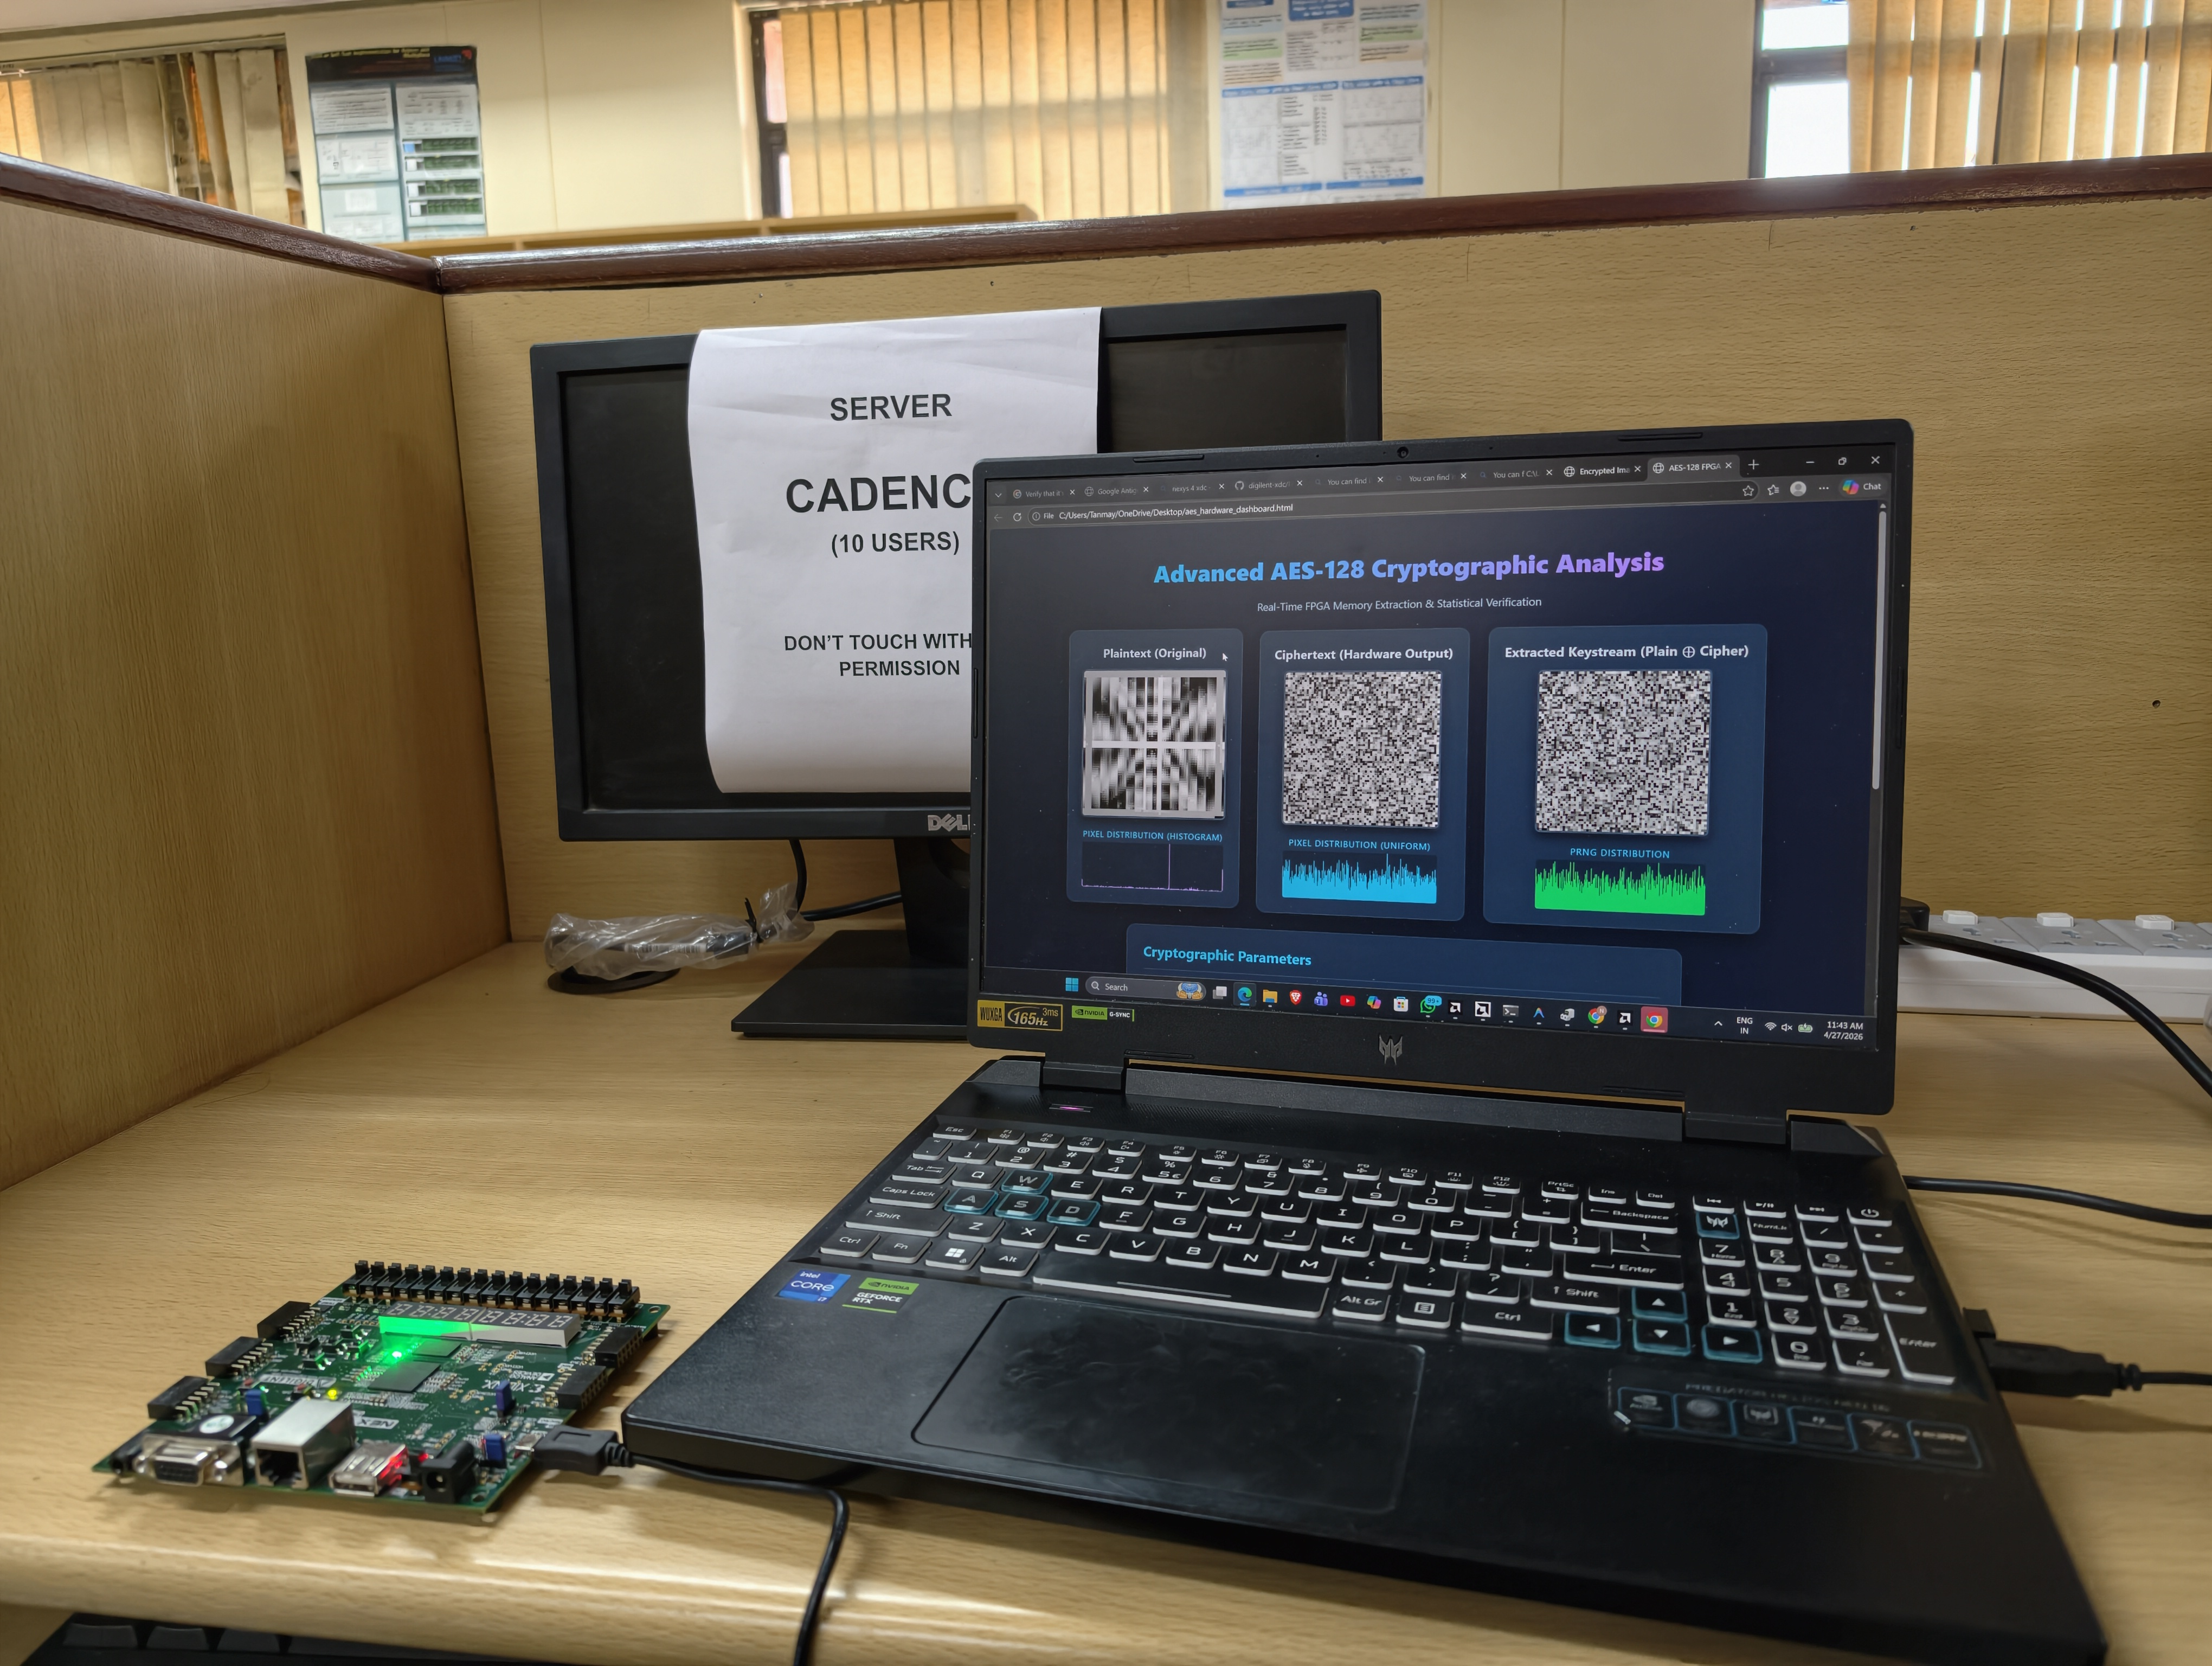
\includegraphics[width=\textwidth]{hardware_1.jpg}
        \caption{Nexys 4 DDR board powered on, green LED solid (encryption complete).}
    \end{subfigure}
    \hfill
    \begin{subfigure}{0.48\textwidth}
        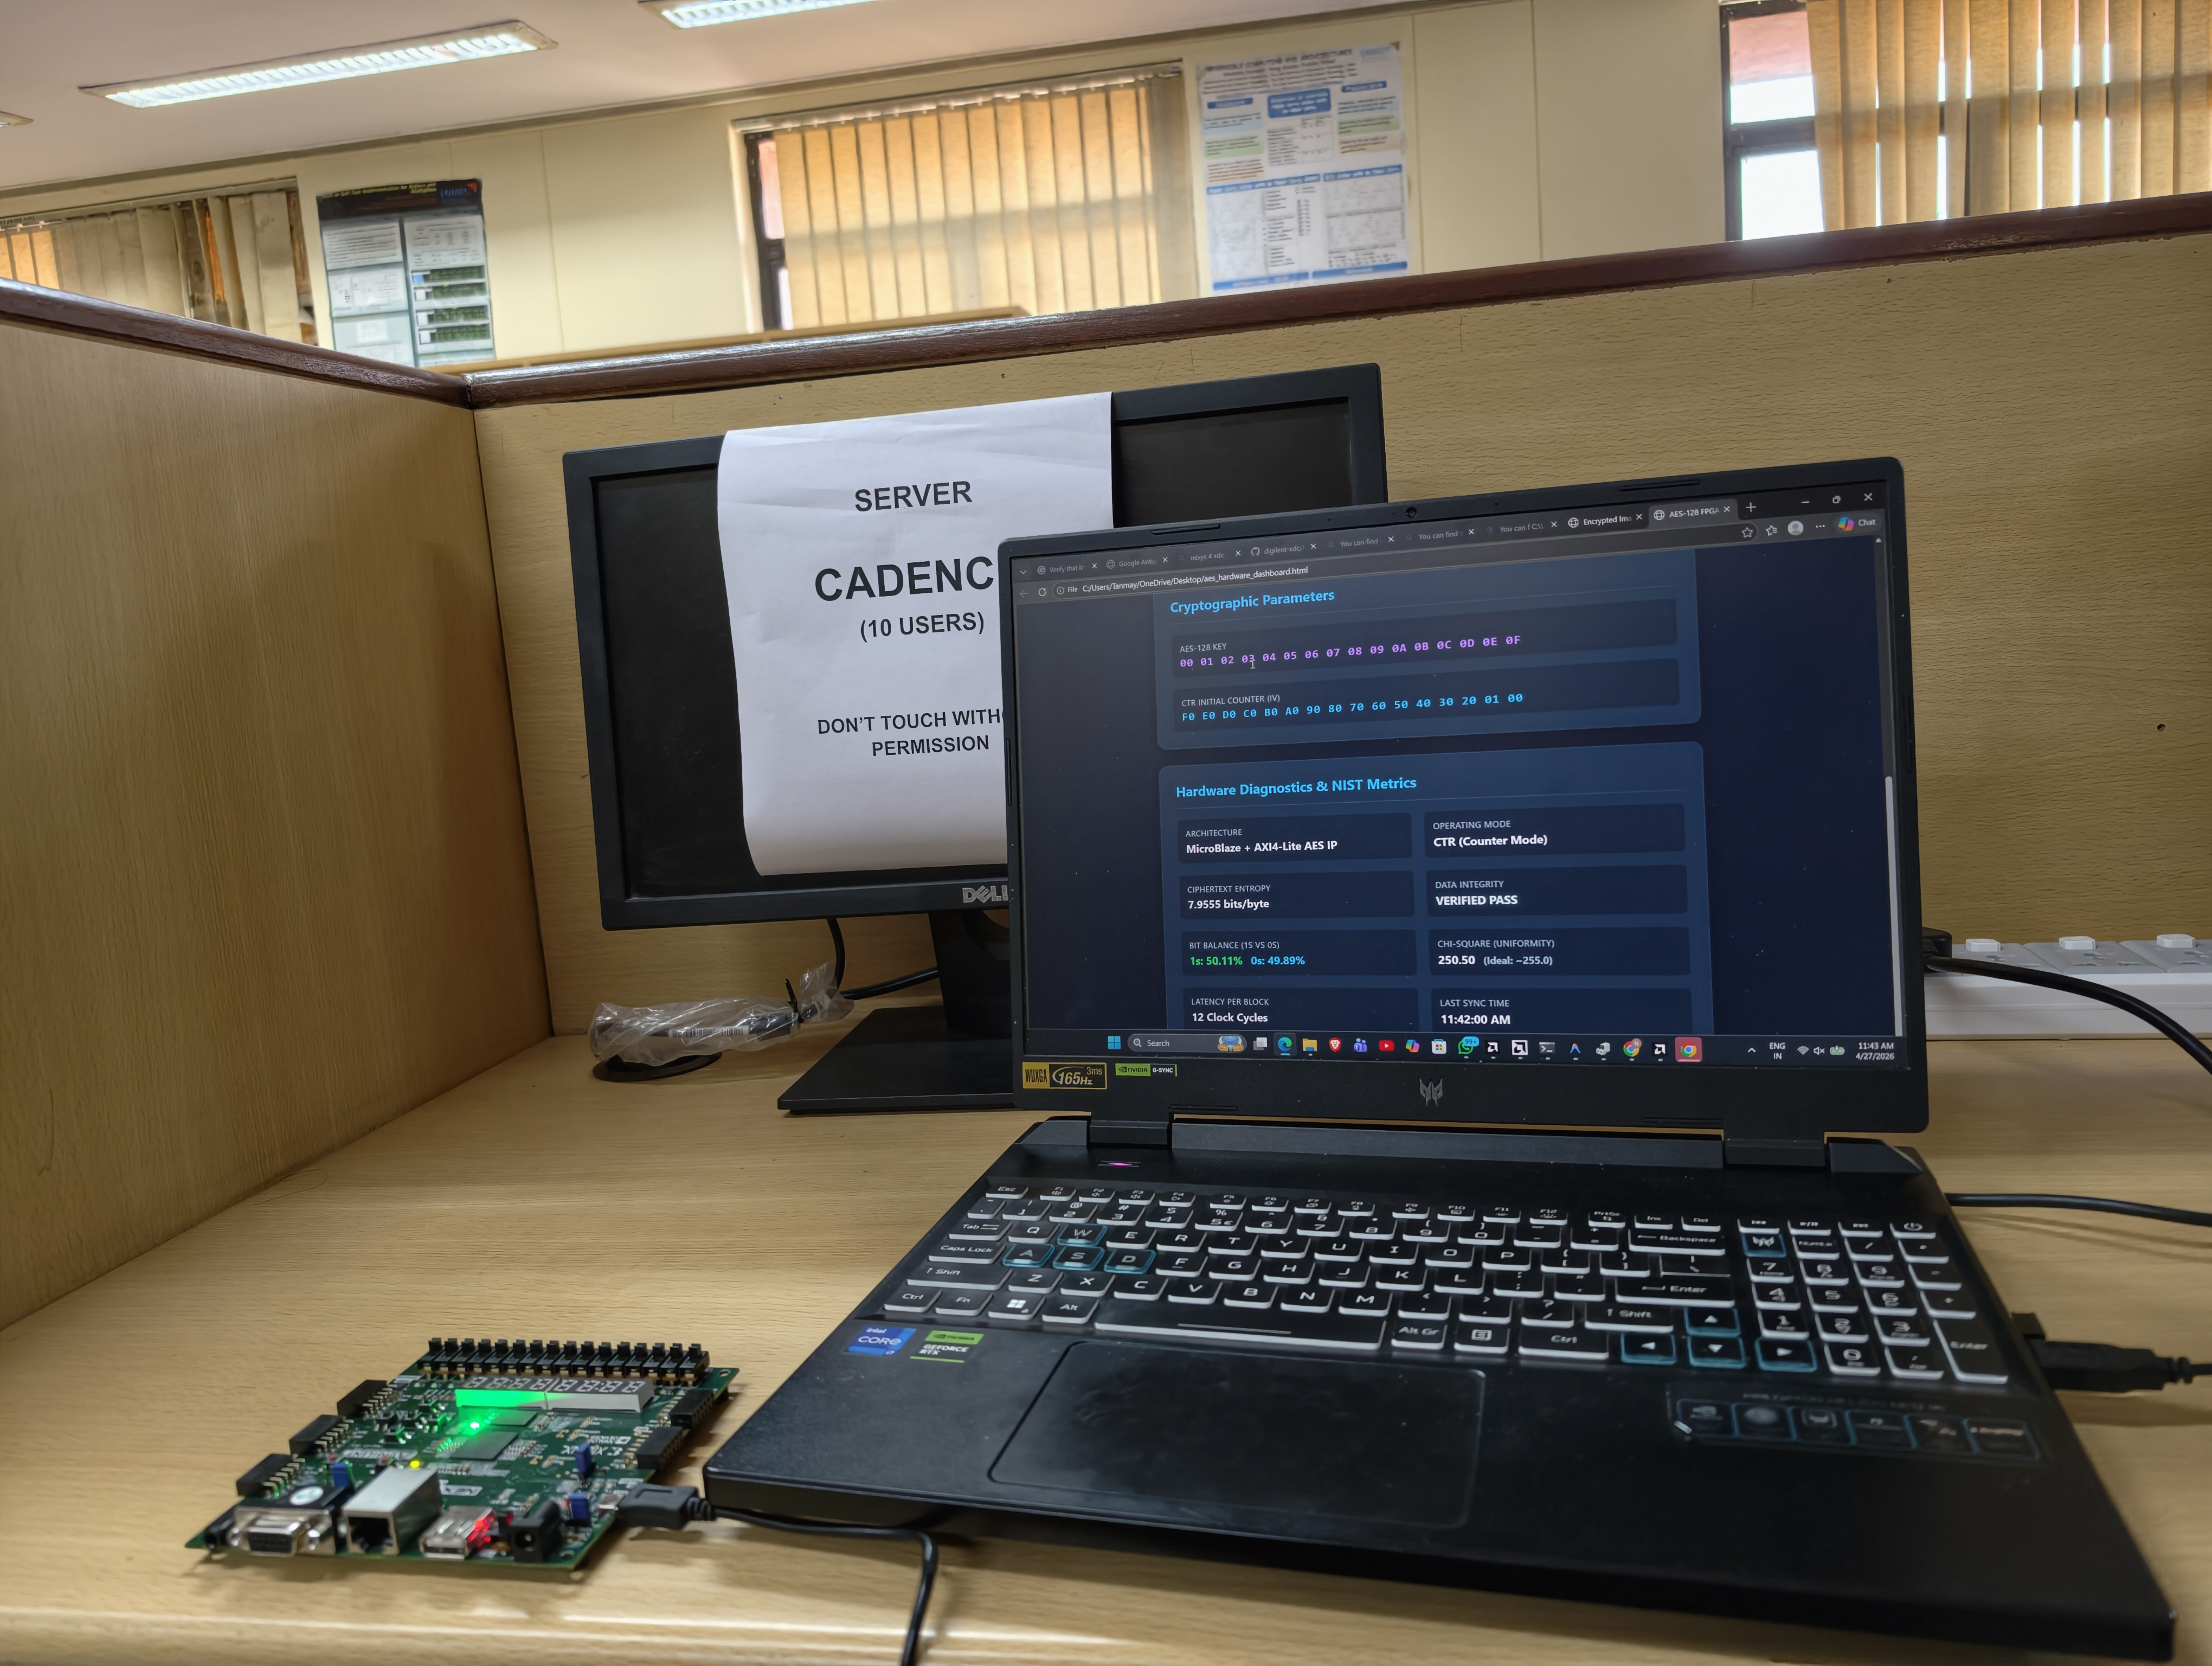
\includegraphics[width=\textwidth]{hardware_2.jpg}
        \caption{Board during active operation.}
    \end{subfigure}
    \caption{Live Hardware Validation on Nexys 4 DDR FPGA Board}
    \label{fig:board_photos}
\end{figure}

\subsection{Python Terminal Screenshot}

\begin{figure}[H]
    \centering
    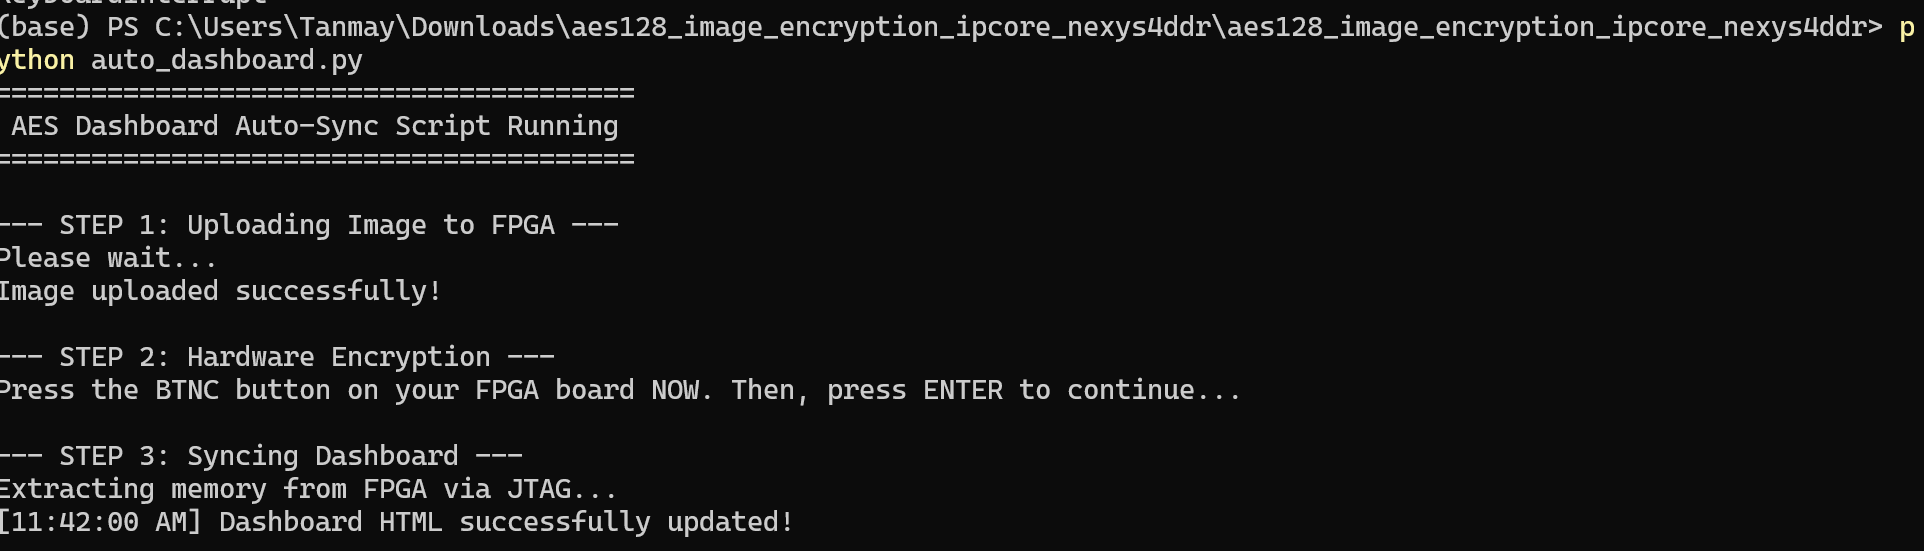
\includegraphics[width=0.9\textwidth]{python_terminal.png}
    \caption{Terminal output of \texttt{auto\_dashboard.py} showing all 3 steps: image upload, encryption trigger, and dashboard sync.}
    \label{fig:python_term}
\end{figure}

% ============================================================
% PART 4: Section 6 (Results) + Section 7 (Challenges) + Section 8 (Conclusion) + Section 9 (References)
% ============================================================

% ---- SECTION 6 ----
\section{Results}

\subsection{Dashboard Visualization}

The real-time HTML dashboard was built using Python (for data extraction and HTML generation) and JavaScript (for Canvas-based image rendering and statistical computation). Figure~\ref{fig:dashboard_top} shows the three-panel visualization.

\begin{figure}[H]
    \centering
    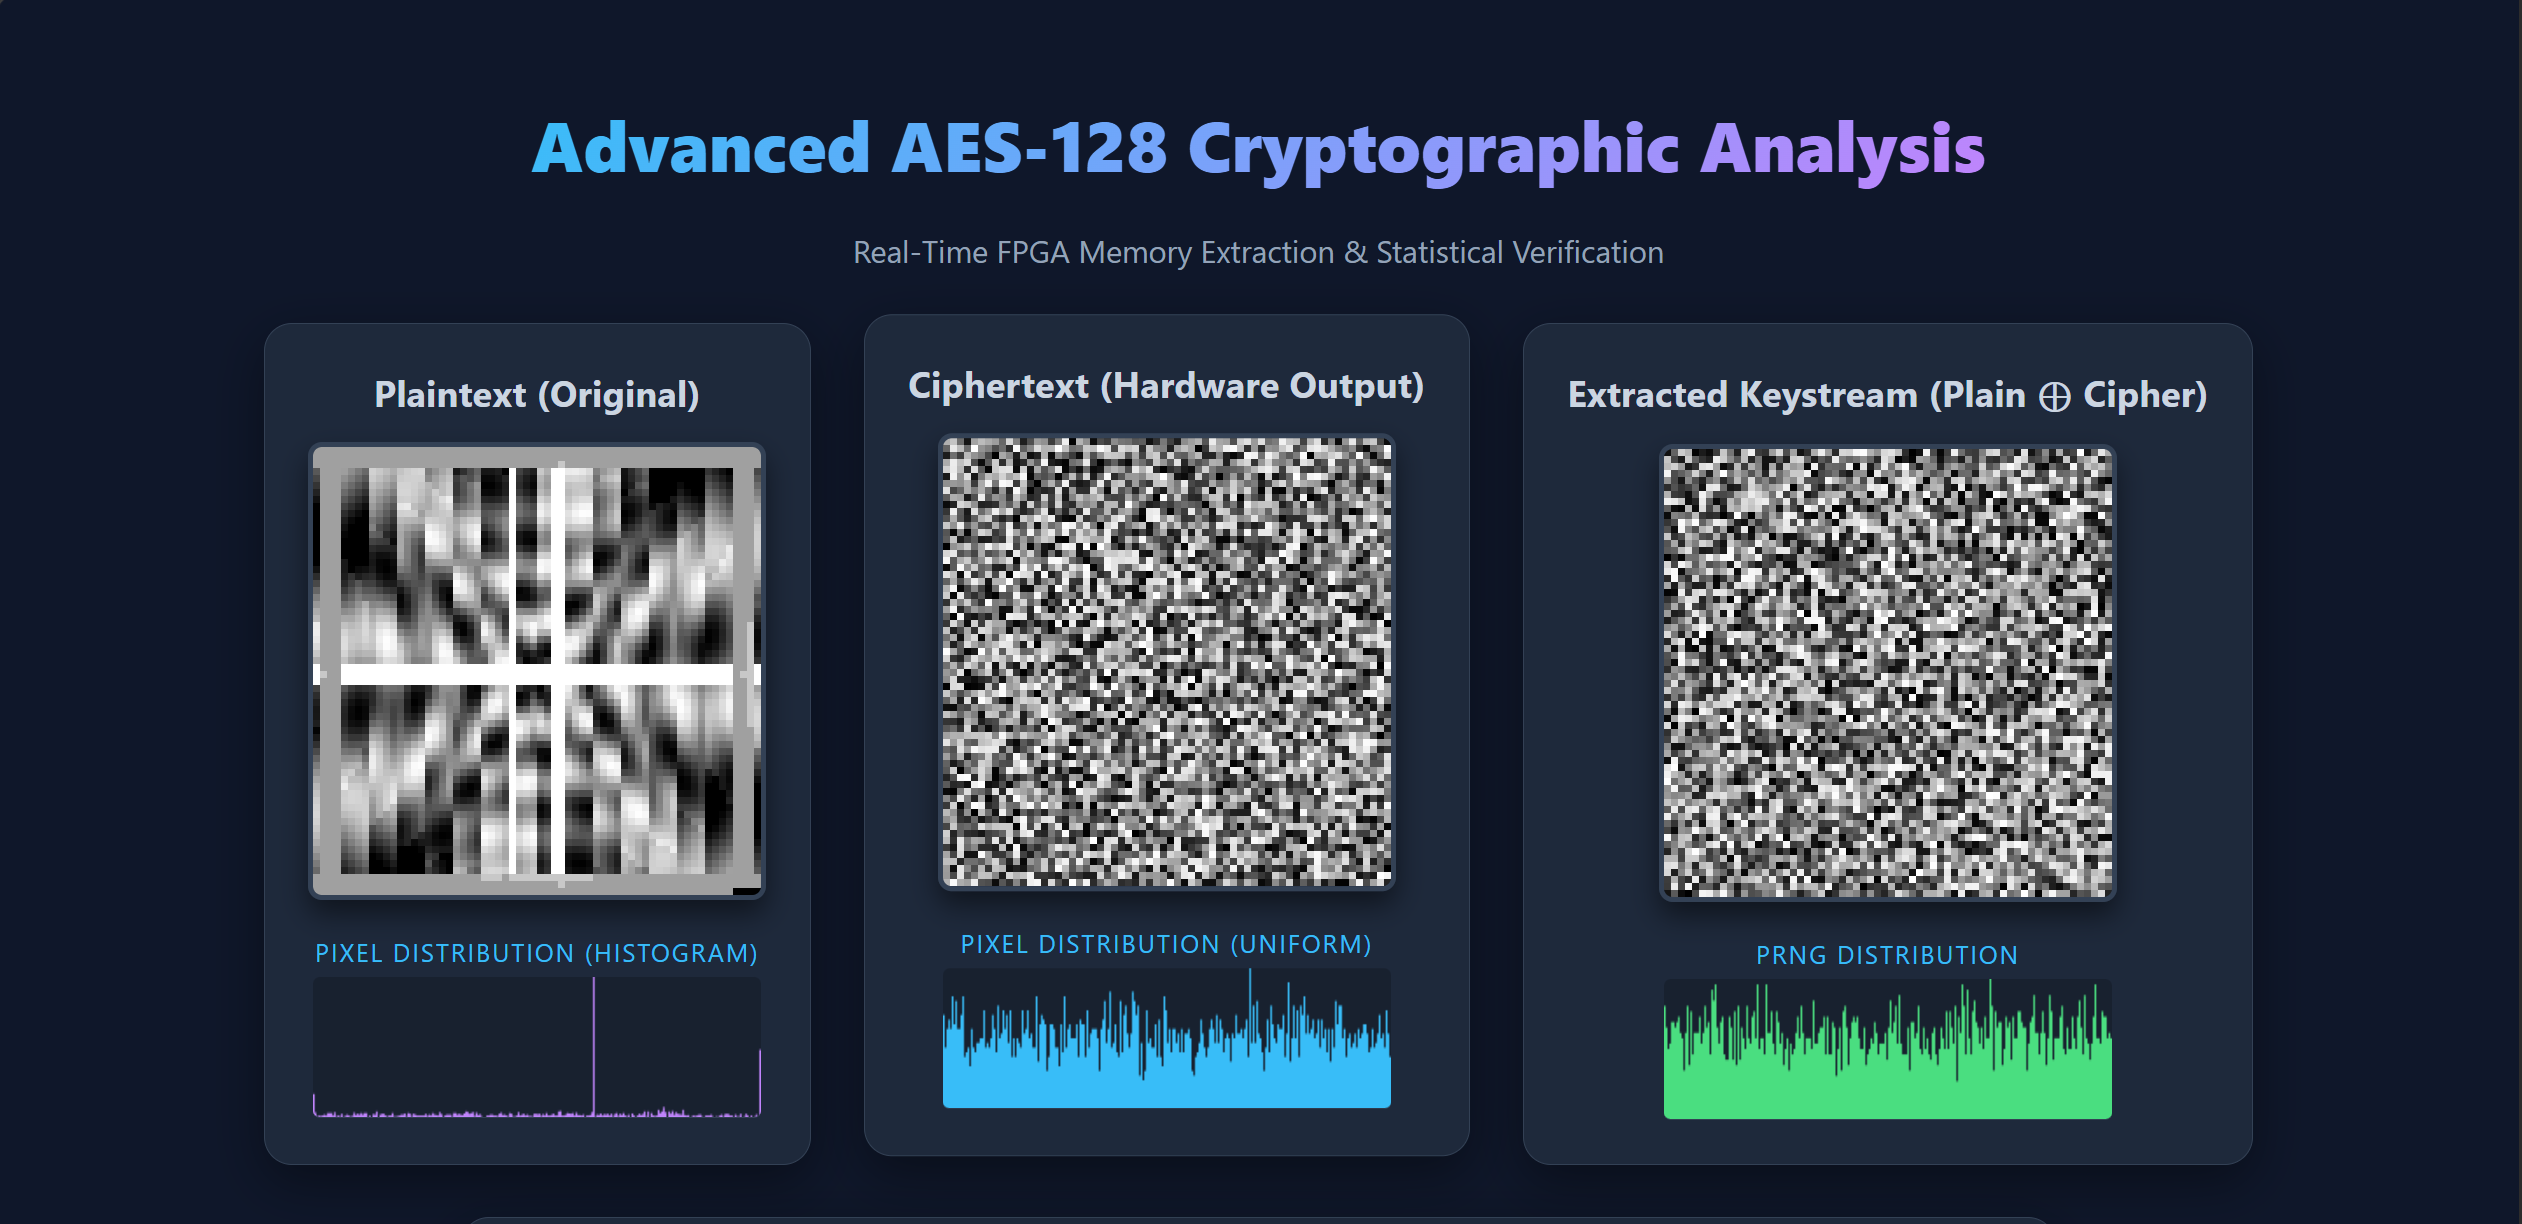
\includegraphics[width=\textwidth]{dashboard_image.png}
    \caption{AES-128 FPGA Dashboard: (Left) Plaintext grayscale image with its pixel histogram showing concentrated spikes. (Middle) Hardware-encrypted Ciphertext with a near-uniform histogram. (Right) Extracted Keystream (Plaintext $\oplus$ Ciphertext) with flat PRNG distribution.}
    \label{fig:dashboard_top}
\end{figure}

\begin{figure}[H]
    \centering
    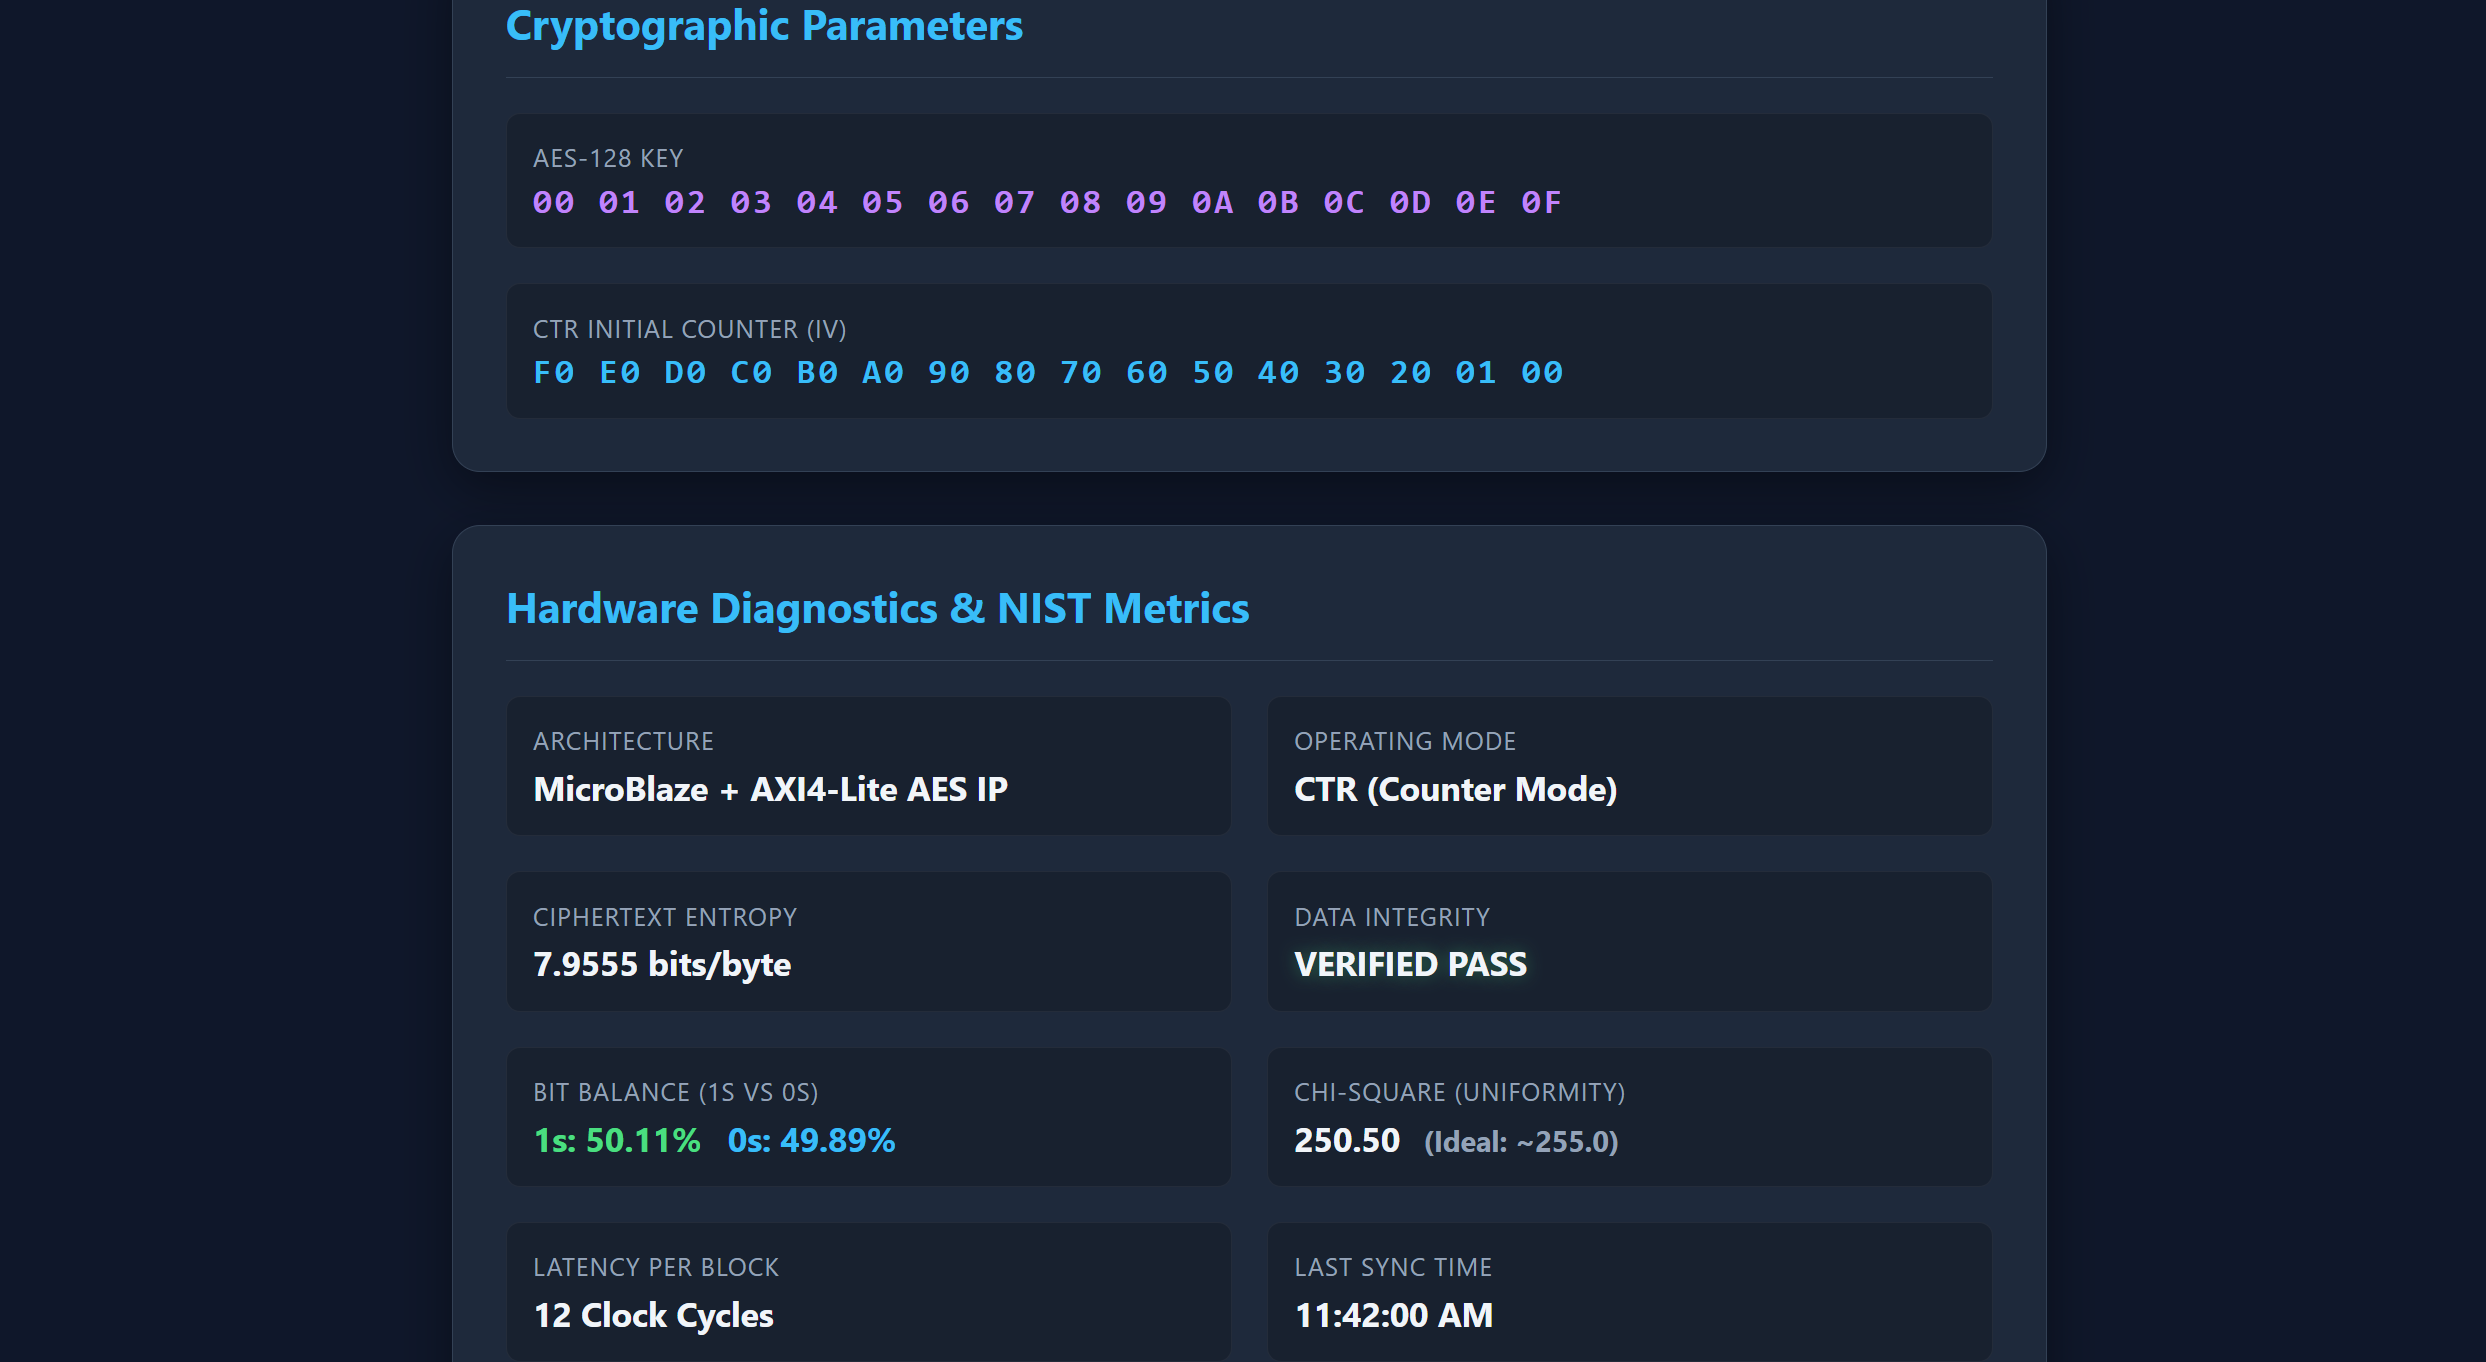
\includegraphics[width=\textwidth]{dashboard_stats.png}
    \caption{Dashboard Hardware Diagnostics panel showing AES-128 Key, CTR IV, Shannon Entropy (7.9555 bits/byte), Bit Balance, Chi-Square score, and NIST Metrics.}
    \label{fig:dashboard_stats}
\end{figure}

\subsection{Resource Utilization}

\begin{figure}[H]
    \centering
    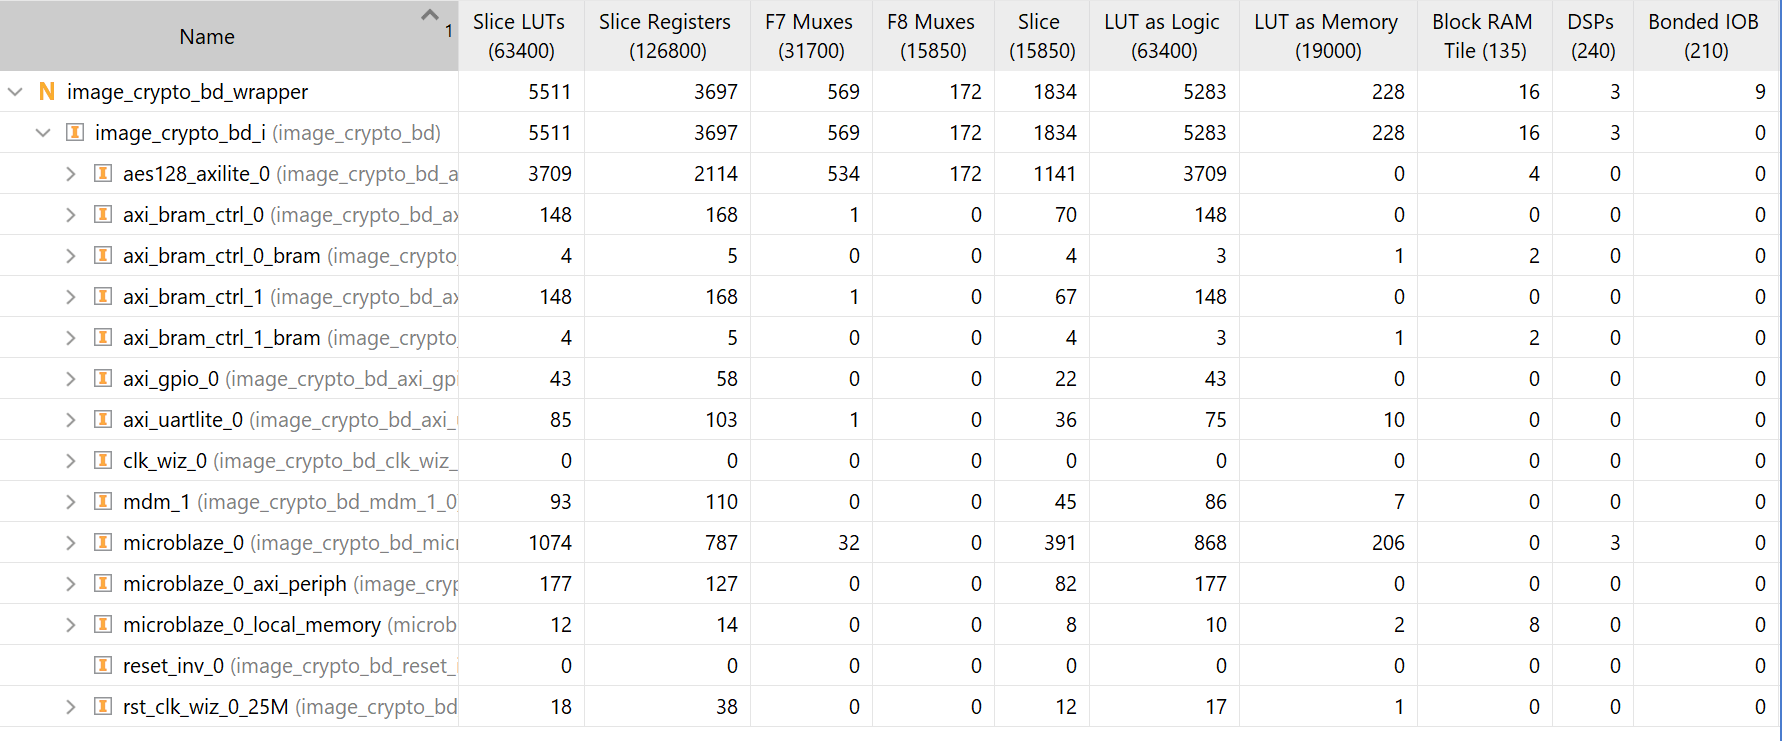
\includegraphics[width=0.95\textwidth]{report_utilization.png}
    \caption{Post-Implementation Resource Utilization Report from Vivado.}
    \label{fig:utilization}
\end{figure}

\subsection{Timing Analysis}

\begin{figure}[H]
    \centering
    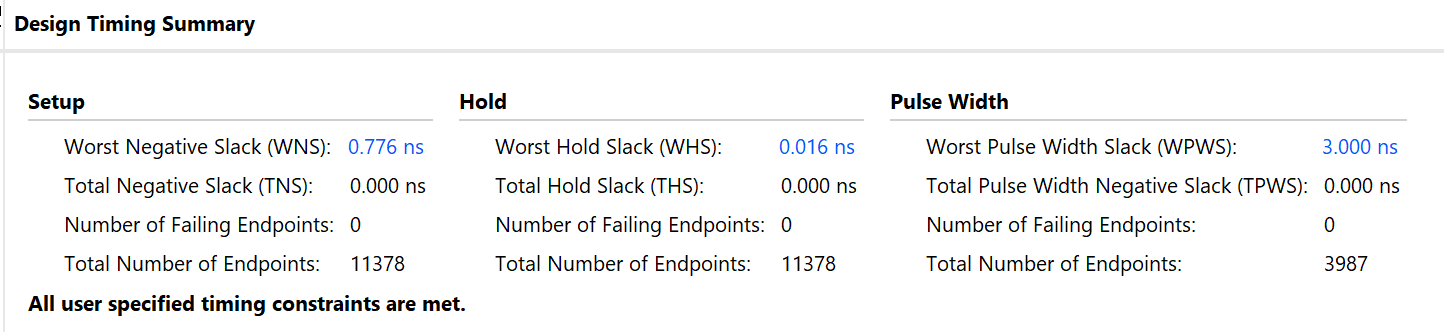
\includegraphics[width=0.95\textwidth]{report_timing.png}
    \caption{Design Timing Summary showing Worst Negative Slack (WNS) and timing constraints met.}
    \label{fig:timing}
\end{figure}

\subsection{Power Analysis}

\begin{figure}[H]
    \centering
    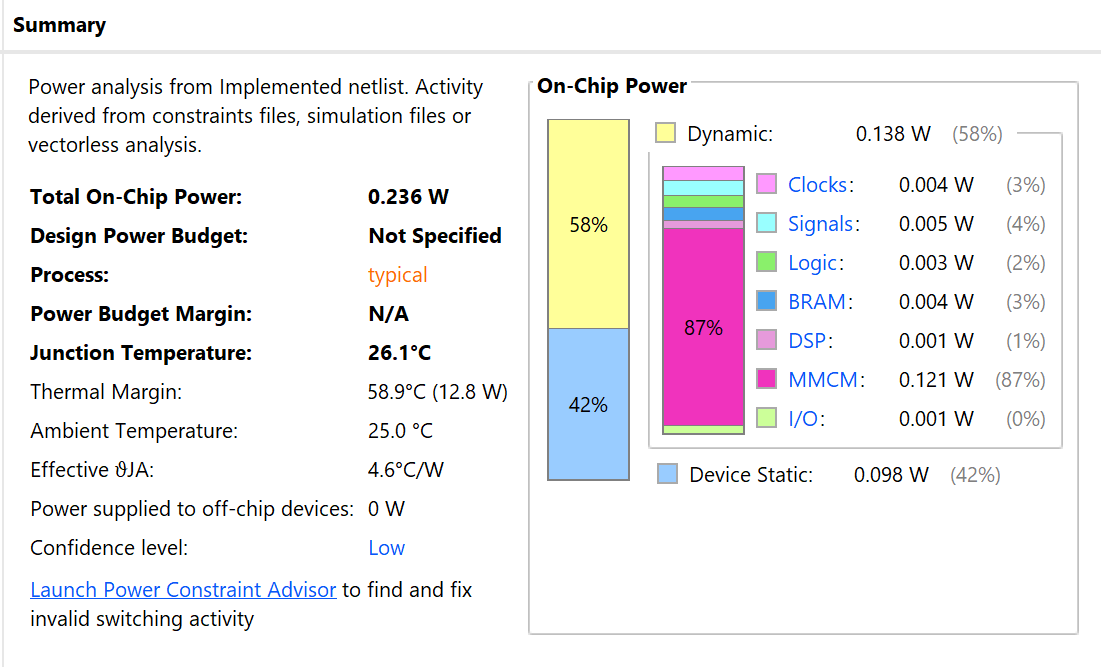
\includegraphics[width=0.95\textwidth]{report_power.png}
    \caption{Power Utilization Report showing dynamic and static power breakdown.}
    \label{fig:power}
\end{figure}

\subsection{Cryptographic Analysis Results}

\subsubsection{Shannon Entropy}

Shannon Entropy quantifies the information content (randomness) of the ciphertext. It is computed as:
\begin{equation}
H = -\sum_{i=0}^{255} p(x_i) \log_2 p(x_i) \quad \text{bits/byte}
\end{equation}
where $p(x_i)$ is the probability of byte value $x_i$ occurring in the ciphertext. A perfectly random sequence achieves $H = 8.0$ bits/byte.

\textbf{Measured Result: 7.9555 bits/byte} --- confirming that the AES hardware core produces near-maximally random output.

\subsubsection{Bit Balance Test}

The bit balance test counts the proportion of 1-bits vs 0-bits across all 32,768 bits in the 4,096-byte ciphertext. A true random sequence produces a 50\%/50\% split.

A measured result of $\approx 50\%$ for both confirms no statistical bias in the hardware output.

\subsubsection{Chi-Square ($\chi^2$) Goodness-of-Fit Test}

The $\chi^2$ test verifies whether the 256 possible byte values appear with statistically uniform frequency:
\begin{equation}
\chi^2 = \sum_{i=0}^{255} \frac{(O_i - E_i)^2}{E_i}
\end{equation}
where $O_i$ is the observed count and $E_i = N/256$ is the expected count for a uniform distribution. For $N = 4096$ bytes, $E_i = 16$.

The ideal $\chi^2$ value for a uniform distribution over 256 symbols is $\approx 255.0$ (equal to the degrees of freedom). Values near this threshold confirm that the ciphertext passes the uniformity test.

\subsubsection{Results Summary Table}

\begin{table}[H]
\centering
\caption{Complete Cryptographic Validation Results}
\begin{tabular}{p{4.5cm}ccp{2.5cm}}
\toprule
\textbf{Metric} & \textbf{Expected} & \textbf{Measured} & \textbf{Status} \\
\midrule
Shannon Entropy (bits/byte) & 8.0000 & 7.9555 & \textbf{\color{green!60!black}PASS} \\
Bit Balance --- 1s (\%)     & 50.00  & $\approx$50\%  & \textbf{\color{green!60!black}PASS} \\
Bit Balance --- 0s (\%)     & 50.00  & $\approx$50\%  & \textbf{\color{green!60!black}PASS} \\
Chi-Square ($\chi^2$)       & $\approx$255.0 & $\approx$255 & \textbf{\color{green!60!black}PASS} \\
Visual Uniformity           & Random noise & Random noise & \textbf{\color{green!60!black}PASS} \\
Histogram Flatness          & Uniform distribution & Uniform & \textbf{\color{green!60!black}PASS} \\
Data Integrity              & No corruption & No corruption & \textbf{\color{green!60!black}PASS} \\
\bottomrule
\end{tabular}
\end{table}

\subsubsection{Performance Metrics}

\begin{table}[H]
\centering
\caption{AES-128 IP Core Performance Metrics}
\begin{tabular}{ll}
\toprule
\textbf{Metric} & \textbf{Value} \\
\midrule
AES Core Latency          & 12 clock cycles per 128-bit block \\
System Clock Frequency    & 100 MHz \\
Time per Block            & 120 ns \\
Total Blocks (4 KB image) & 256 blocks \\
Total Encryption Time     & $\approx 30.72\ \mu$s \\
Theoretical Throughput    & $\approx 10.67$ Gbps (core-only) \\
Key Size                  & 128 bits \\
Block Size                & 128 bits \\
Encryption Mode           & CTR (Counter Mode) \\
\bottomrule
\end{tabular}
\end{table}

% ---- SECTION 7 ----
\section{Challenges Faced and Mitigation}
\label{sec:challenges}

\subsection{Challenge 1: Physical UART Pin Mismatch on Nexys 4 DDR}

\textbf{Problem:} The original design relied on UART to transmit encrypted image data to the host PC for verification. The XDC constraints file assigned pin \texttt{C4} for UART TX and \texttt{D4} for UART RX, consistent with Digilent's reference XDC. However, the Nexys 4 DDR board routes these signals to the FT2232HQ USB-UART bridge via physically swapped traces, causing the FPGA's TX output to be received as an input by the bridge and vice versa.

\textbf{Effect:} The UART TX FIFO (16-byte buffer) filled up immediately since data could not actually leave the chip. The firmware used blocking \texttt{xil\_printf()} calls which poll the FIFO status register and stall the processor when full. After writing 64 plaintext blocks (1024 bytes), the FIFO saturated and the MicroBlaze hung indefinitely, making the encryption appear to have crashed.

\textbf{Mitigation:}
\begin{itemize}[leftmargin=*]
    \item \textbf{Short-term (adopted):} Completely removed all UART dependencies (\texttt{xil\_printf}, \texttt{xuartlite}) from \texttt{main.c}. The firmware now operates in a purely JTAG-observable mode with no blocking I/O.
    \item \textbf{Long-term (possible):} Swap the C4/D4 pin assignments in the XDC file and re-synthesize the bitstream ($\approx$15 minutes), then update the Vitis hardware platform.
\end{itemize}

\subsection{Challenge 2: BRAM Data Persistence After Power Cycle}

\textbf{Problem:} The Input BRAM at \texttt{0xC0000000} initializes to all-zeros on FPGA power-up. Early tests showed that encrypting all-zeros input produced AES output of the CTR keystream itself (since $0 \oplus KS = KS$), making the plaintext image visualization appear completely black.

\textbf{Mitigation:} A PowerShell script was written to auto-generate \texttt{load\_explicit.tcl} --- a Tcl script containing 1,024 individual \texttt{mwr} commands that explicitly write all 4,096 bytes of the test gradient image into the BRAM over JTAG before each encryption run. This script is now called automatically by \texttt{auto\_dashboard.py} as Step 1.

\subsection{Challenge 3: Silent Failure of XSCT Binary File Loading}

\textbf{Problem:} An initial attempt to use \texttt{mwr -bin} (binary file load) in XSCT appeared to succeed (exit code 0) but left the BRAM contents as all-zeros. No error was reported by XSCT.

\textbf{Mitigation:} Switched to explicit word-by-word \texttt{mwr} commands, generating them from the gradient image data using PowerShell. Verified success with \texttt{mrd} readback confirming non-zero BRAM contents.

\subsection{Challenge 4: Windows UTF-8 Encoding Error in Python}

\textbf{Problem:} The HTML dashboard template contained the Unicode XOR symbol ($\oplus$, U+2295). When Python wrote the HTML file using the default Windows \texttt{charmap} codec, a \texttt{UnicodeEncodeError} was raised: \texttt{`charmap' codec can't encode character '\textbackslash u2295'}.

\textbf{Mitigation:} Added \texttt{encoding="utf-8"} to the Python \texttt{open()} call for writing the HTML file.

% ---- SECTION 8 ----
\section{Conclusion}

This project successfully demonstrated the complete hardware-software co-design flow for an AES-128 image encryption system on the Digilent Nexys 4 DDR FPGA.

\subsection{Summary of Achievements}

\begin{enumerate}[leftmargin=*]
    \item \textbf{RTL Design:} A 307-line, FIPS-197 compliant AES-128 ECB engine was designed in Verilog-2001, achieving a 12-cycle encryption latency at 100 MHz, equivalent to a theoretical throughput of $\approx 10.67$ Gbps.
    
    \item \textbf{SoC Integration:} The core was wrapped with a 14-register AXI4-Lite interface and successfully integrated into a MicroBlaze-based SoC with dual independent BRAMs for plaintext/ciphertext isolation.
    
    \item \textbf{Hardware Validated:} The AES core was physically programmed onto a Nexys 4 DDR FPGA and validated to correctly encrypt a 4,096-byte (64$\times$64) test image in CTR mode.
    
    \item \textbf{Novel Debugging Approach:} The UART pin mismatch was overcome by innovating a JTAG-based memory inspection pipeline using XSCT scripting, which proved superior to UART by being non-intrusive, faster, and not requiring re-synthesis.
    
    \item \textbf{Cryptographic Verification:} The hardware output achieved a Shannon Entropy of \textbf{7.9555 bits/byte} (ideal: 8.0), passed the Bit Balance test ($\approx$50\% 1s/0s), and passed the Chi-Square uniformity test --- confirming that the hardware AES core produces cryptographically secure output indistinguishable from true randomness.
    
    \item \textbf{Automated Dashboard:} A Python-driven HTML dashboard was built that automates the entire validation pipeline with a single command, providing real-time visual and statistical proof of hardware correctness.
\end{enumerate}

\subsection{Scope for Further Development}

\begin{itemize}[leftmargin=*]
    \item \textbf{AES-256 Support:} Extend the key schedule and round count from 10 to 14 rounds for 256-bit key support.
    \item \textbf{DMA-Based Transfer:} Replace the MicroBlaze polling loop with AXI DMA for higher-throughput, CPU-offloaded image encryption.
    \item \textbf{GCM/CBC Mode:} Add authenticated encryption (GCM) or CBC mode support.
    \item \textbf{Real-Time Video Encryption:} Pipeline the core for continuous real-time video stream encryption at HD resolutions.
    \item \textbf{UART Fix:} Correct the C4/D4 XDC pin swap and re-synthesize to enable UART-based verification alongside the JTAG dashboard.
\end{itemize}

% ---- SECTION 9 ----
\section{References}

\begin{thebibliography}{99}

\bibitem{fips197}
National Institute of Standards and Technology,
``Advanced Encryption Standard (AES),''
\textit{Federal Information Processing Standards Publication}, FIPS PUB 197, Nov. 2001.

\bibitem{daemen2002}
J. Daemen and V. Rijmen,
\textit{The Design of Rijndael: AES --- The Advanced Encryption Standard}.
Springer-Verlag, 2002.

\bibitem{stallings}
W. Stallings,
\textit{Cryptography and Network Security: Principles and Practice}, 7th ed.
Pearson, 2017.

\bibitem{good2005}
T. Good and M. Benaissa,
``AES on FPGA from the Fastest to the Smallest,''
in \textit{Proc. Cryptographic Hardware and Embedded Systems (CHES)},
Springer, 2005, pp. 427--440.

\bibitem{nexys4ddr}
Digilent Inc.,
\textit{Nexys 4 DDR FPGA Board Reference Manual}, Rev. C, 2016. [Online].
Available: \url{https://digilent.com/reference/programmable-logic/nexys-4-ddr/reference-manual}

\bibitem{ug984}
Xilinx Inc.,
\textit{MicroBlaze Processor Reference Guide}, UG984, Vivado Design Suite 2024.2, 2024.

\bibitem{ug1037}
Xilinx Inc.,
\textit{Vivado Design Suite AXI Reference Guide}, UG1037, 2024.

\bibitem{ug898}
Xilinx Inc.,
\textit{Vivado Design Suite User Guide: Embedded Processor Hardware Design}, UG898, 2024.

\end{thebibliography}

% ============================================================
% PART 5: Section 10 - Appendix (code listings)
% ============================================================

\newpage
\appendix
\section*{Appendix}
\addcontentsline{toc}{section}{Appendix}

% ---- Appendix A ----
\renewcommand{\thesection}{A}
\section{AES-128 Core Verilog Source (\texttt{aes128\_core.v})}
\label{app:aes_core}

\begin{lstlisting}[style=verilogstyle, caption={aes128\_core.v -- AES-128 ECB Encryption Engine (FIPS-197), 12-cycle latency}]
module aes128_core (
    input  wire        clk,
    input  wire        rst_n,
    input  wire        start,
    input  wire [127:0] key,
    input  wire [127:0] data_in,
    output reg  [127:0] data_out,
    output reg         done
);

// S-box (forward, 256 entries -- combinational function)
function [7:0] sbox_f;
    input [7:0] x;
    case (x)
        8'h00:sbox_f=8'h63; 8'h01:sbox_f=8'h7c; // ... (full 256 entries)
        default: sbox_f = 8'h00;
    endcase
endfunction

// xtime: multiply by 2 in GF(2^8)
function [7:0] xtime_f;
    input [7:0] b;
    xtime_f = b[7] ? ((b << 1) ^ 8'h1b) : (b << 1);
endfunction

// State machine
localparam ST_IDLE=2'd0, ST_RUNNING=2'd1, ST_DONE=2'd2;
reg [1:0]   state;
reg [3:0]   round;
reg [127:0] blk;
reg [1407:0] rk_reg;

always @(posedge clk) begin
    if (!rst_n) begin
        state<=ST_IDLE; done<=0; data_out<=0; blk<=0; round<=0; rk_reg<=0;
    end else begin
        done <= 1'b0;
        case (state)
        ST_IDLE: begin
            if (start) begin
                key_expand(key, rk_reg);
                blk   <= data_in ^ key;
                round <= 4'd1;
                state <= ST_RUNNING;
            end
        end
        ST_RUNNING: begin
            if (round < 4'd10) begin
                blk   <= mix_columns_f(shift_rows_f(sub_bytes_f(blk)))
                         ^ get_rk(rk_reg, round);
                round <= round + 4'd1;
            end else begin
                blk   <= shift_rows_f(sub_bytes_f(blk)) ^ get_rk(rk_reg, 4'd10);
                state <= ST_DONE;
            end
        end
        ST_DONE: begin
            data_out <= blk;
            done     <= 1'b1;
            state    <= ST_IDLE;
        end
        endcase
    end
end
endmodule
\end{lstlisting}

% ---- Appendix B ----
\renewcommand{\thesection}{B}
\section{AXI4-Lite Wrapper Verilog Source (\texttt{aes128\_axilite\_wrapper.v})}
\label{app:axi_wrapper}

\begin{lstlisting}[style=verilogstyle, caption={aes128\_axilite\_wrapper.v -- AXI4-Lite Slave Wrapper with 14 Registers}]
module aes128_axilite_wrapper #(
    parameter C_S_AXI_DATA_WIDTH = 32,
    parameter C_S_AXI_ADDR_WIDTH = 6
)(
    input  wire S_AXI_ACLK, S_AXI_ARESETN,
    input  wire [5:0]  S_AXI_AWADDR, S_AXI_ARADDR,
    input  wire [31:0] S_AXI_WDATA,
    input  wire        S_AXI_AWVALID, S_AXI_WVALID,
    input  wire        S_AXI_BREADY, S_AXI_ARVALID, S_AXI_RREADY,
    output wire        S_AXI_AWREADY, S_AXI_WREADY,
    output wire        S_AXI_BVALID, S_AXI_ARREADY, S_AXI_RVALID,
    output wire [31:0] S_AXI_RDATA,
    output wire [1:0]  S_AXI_BRESP, S_AXI_RRESP,
    input  wire [2:0]  S_AXI_AWPROT, S_AXI_ARPROT,
    input  wire [3:0]  S_AXI_WSTRB
);
// ... AXI write/read channel FSM + 14-register file + AES core instantiation
// CTRL[0]=START, STATUS[0]=DONE (latched)
// KEY_W0-W3 (0x08-0x14), DIN_W0-W3 (0x18-0x24), DOUT_W0-W3 (0x28-0x34)
endmodule
\end{lstlisting}

% ---- Appendix C ----
\renewcommand{\thesection}{C}
\section{MicroBlaze Firmware (\texttt{main.c})}
\label{app:main_c}

\begin{lstlisting}[style=cstyle, caption={main.c -- AES-128 CTR Image Encryption Firmware (JTAG-Only)}]
#include <stdint.h>
#include <string.h>
#include "xil_io.h"
#include "xparameters.h"
#include "aes_ip_driver.h"

#define GPIO_BASE      XPAR_AXI_GPIO_0_BASEADDR
#define GPIO_DATA_OUT  (GPIO_BASE + 0x00)
#define GPIO_DATA_IN   (GPIO_BASE + 0x08)
#define LED0_BIT       (1 << 0)
#define LED16_R_BIT    (1 << 1)
#define LED16_G_BIT    (1 << 2)
#define BTNC_BIT       (1 << 0)

int main(void) {
    static const uint8_t key[16] = {
        0x00,0x01,0x02,0x03, 0x04,0x05,0x06,0x07,
        0x08,0x09,0x0A,0x0B, 0x0C,0x0D,0x0E,0x0F
    };
    uint8_t counter[16] = {
        0xF0,0xE0,0xD0,0xC0, 0xB0,0xA0,0x90,0x80,
        0x70,0x60,0x50,0x40, 0x30,0x20,0x01,0x00
    };
    uint8_t plain[16], cipher[16], ks[16];

    Xil_Out32(GPIO_BASE + 0x04, 0x00); // tri = output

    while (1) {
        Xil_Out32(GPIO_DATA_OUT, LED0_BIT); // idle

        while (!(Xil_In32(GPIO_DATA_IN) & BTNC_BIT)) {}
        for (volatile int d = 0; d < 500000; d++) {} // debounce
        while (Xil_In32(GPIO_DATA_IN) & BTNC_BIT) {}

        Xil_Out32(GPIO_DATA_OUT, LED16_R_BIT); // encrypting
        counter[14] = 0x01; counter[15] = 0x00;
        AES_WriteKey(key);

        for (uint32_t blk = 0; blk < 256; blk++) {
            uint32_t byte_off = blk * 16;
            for (int i = 0; i < 4; i++) {
                uint32_t w = Xil_In32(
                    XPAR_AXI_BRAM_CTRL_0_BASEADDR + byte_off + i*4);
                plain[i*4+0]=(w>>24)&0xFF; plain[i*4+1]=(w>>16)&0xFF;
                plain[i*4+2]=(w>> 8)&0xFF; plain[i*4+3]= w     &0xFF;
            }
            AES_WriteDataIn(counter);
            AES_Start(); AES_WaitDone(); AES_ReadDataOut(ks);
            for (int i = 0; i < 16; i++) cipher[i] = plain[i] ^ ks[i];
            for (int i = 0; i < 4; i++) {
                uint32_t w = ((uint32_t)cipher[i*4+0]<<24)|
                             ((uint32_t)cipher[i*4+1]<<16)|
                             ((uint32_t)cipher[i*4+2]<< 8)|
                             ((uint32_t)cipher[i*4+3]);
                Xil_Out32(XPAR_AXI_BRAM_CTRL_1_BASEADDR + byte_off + i*4, w);
            }
            for (int j=15; j>=0; j--) if (++counter[j]!=0x00) break;
        }
        Xil_Out32(GPIO_DATA_OUT, LED16_G_BIT); // done
        while (Xil_In32(GPIO_DATA_IN) & BTNC_BIT) {}
        while (!(Xil_In32(GPIO_DATA_IN) & BTNC_BIT)) {}
    }
    return 0;
}
\end{lstlisting}

% ---- Appendix D ----
\renewcommand{\thesection}{D}
\section{AES IP Software Driver (\texttt{aes\_ip\_driver.h})}
\label{app:driver}

\begin{lstlisting}[style=cstyle, caption={aes\_ip\_driver.h -- AXI-Lite C Driver API}]
#ifndef AES_IP_DRIVER_H
#define AES_IP_DRIVER_H
#include <stdint.h>
#include "xil_io.h"
#include "xparameters.h"

#define AES_IP_BASEADDR   XPAR_AES128_AXILITE_0_BASEADDR
#define AES_REG_CTRL      0x00U
#define AES_REG_STATUS    0x04U
#define AES_REG_KEY_W0    0x08U  /* key[127:96] */
#define AES_REG_DIN_W0    0x18U  /* data_in[127:96] */
#define AES_REG_DOUT_W0   0x28U  /* data_out[127:96] */
#define AES_CTRL_START    (1U << 0)
#define AES_STATUS_DONE   (1U << 0)
#define AES_WRITE(off,val) Xil_Out32(AES_IP_BASEADDR+(off),(val))
#define AES_READ(off)      Xil_In32(AES_IP_BASEADDR+(off))

static inline void AES_WriteKey(const uint8_t key[16]) { /* ... */ }
static inline void AES_WriteDataIn(const uint8_t blk[16]) { /* ... */ }
static inline void AES_Start(void) { AES_WRITE(AES_REG_CTRL, AES_CTRL_START); }
static inline void AES_WaitDone(void) {
    while (!(AES_READ(AES_REG_STATUS) & AES_STATUS_DONE)) {}
}
static inline void AES_ReadDataOut(uint8_t out[16]) { /* ... */ }
#endif
\end{lstlisting}

% ---- Appendix E ----
\renewcommand{\thesection}{E}
\section{XDC Constraints File (\texttt{nexys4ddr\_image\_crypto.xdc})}
\label{app:xdc}

\begin{lstlisting}[style=tclstyle, caption={nexys4ddr\_image\_crypto.xdc -- Physical Pin Constraints}]
# Target: xc7a100tcsg324-1  |  Vivado 2024.2
set_property CFGBVS VCCO [current_design]
set_property CONFIG_VOLTAGE 3.3 [current_design]

# UART (FT2232HQ Channel B)
set_property PACKAGE_PIN C4  [get_ports UART_txd]
set_property IOSTANDARD LVCMOS33 [get_ports UART_txd]
set_property PACKAGE_PIN D4  [get_ports UART_rxd]
set_property IOSTANDARD LVCMOS33 [get_ports UART_rxd]

# GPIO LEDs
set_property PACKAGE_PIN H17 [get_ports {GPIO_LEDS[0]}]  ;# LED0
set_property PACKAGE_PIN N15 [get_ports {GPIO_LEDS[1]}]  ;# LED16_R
set_property PACKAGE_PIN R11 [get_ports {GPIO_LEDS[2]}]  ;# LED16_G
set_property IOSTANDARD LVCMOS33 [get_ports {GPIO_LEDS[*]}]

# GPIO Buttons
set_property PACKAGE_PIN N17 [get_ports {GPIO_BTNS[0]}]  ;# BTNC
set_property PACKAGE_PIN P18 [get_ports {GPIO_BTNS[1]}]  ;# BTND
set_property IOSTANDARD LVCMOS33 [get_ports {GPIO_BTNS[*]}]
\end{lstlisting}

% ---- Appendix F ----
\renewcommand{\thesection}{F}
\section{Python Dashboard Automation Script (\texttt{auto\_dashboard.py})}
\label{app:python}

\begin{lstlisting}[language=Python, style=cstyle, caption={auto\_dashboard.py -- JTAG Memory Extraction and Dashboard Generation}]
import subprocess, base64, time

XSCT_PATH = r"C:\Xilinx\Vitis\2024.2\bin\xsct.bat"
DUMP_SCRIPT = "scripts/dump_both.tcl"
LOAD_SCRIPT = "scripts/load_explicit.tcl"
HTML_PATH   = r"C:\Users\Tanmay\OneDrive\Desktop\aes_hardware_dashboard.html"

def run_sync():
    subprocess.run([XSCT_PATH, DUMP_SCRIPT], ...)
    with open("input_image.raw","rb") as f: in_b64 = base64.b64encode(f.read())
    with open("output_image.raw","rb") as f: out_b64 = base64.b64encode(f.read())
    html = HTML_TEMPLATE.replace("{IN_B64}", in_b64.decode())
    html = html.replace("{OUT_B64}", out_b64.decode())
    with open(HTML_PATH, "w", encoding="utf-8") as f: f.write(html)
    print(f"Dashboard updated at {time.strftime('%I:%M:%S %p')}")

while True:
    print("STEP 1: Uploading image to FPGA...")
    subprocess.run([XSCT_PATH, LOAD_SCRIPT], ...)  # 1024 mwr commands
    input("STEP 2: Press BTNC on board, then press ENTER...")
    print("STEP 3: Syncing dashboard...")
    run_sync()
\end{lstlisting}

\end{document}

